%% LyX 1.3 created this file.  For more info, see http://www.lyx.org/.
%% Do not edit unless you really know what you are doing.
\documentclass[english, 12pt]{article}
\usepackage{times}
%\usepackage{algorithm2e}
\usepackage{url}
\usepackage{bbm}
\usepackage[T1]{fontenc}
\usepackage[latin1]{inputenc}
\usepackage{geometry}
\geometry{verbose,letterpaper,tmargin=2cm,bmargin=2cm,lmargin=1.5cm,rmargin=1.5cm}
\usepackage{rotating}
\usepackage{color}
\usepackage{graphicx}
\usepackage{subcaption}
\usepackage{amsmath, amsthm, amssymb}
\usepackage{setspace}
\usepackage{lineno}
\usepackage{hyperref}
\usepackage{bbm}
\usepackage{makecell}

\renewcommand{\arraystretch}{2}

%\usepackage{xr}
%\externaldocument{SCT-supp}

%\linenumbers
%\doublespacing
\onehalfspacing
%\usepackage[authoryear]{natbib}
\usepackage{natbib} \bibpunct{(}{)}{;}{author-year}{}{,}

%Pour les rajouts
\usepackage{color}
\definecolor{trustcolor}{rgb}{0,0,1}

\usepackage{dsfont}
\usepackage[warn]{textcomp}
\usepackage{adjustbox}
\usepackage{multirow}
\usepackage{graphicx}
\graphicspath{{figures/}}
\DeclareMathOperator*{\argmin}{\arg\!\min}

\let\tabbeg\tabular
\let\tabend\endtabular
\renewenvironment{tabular}{\begin{adjustbox}{max width=0.9\textwidth}\tabbeg}{\tabend\end{adjustbox}}

\makeatletter

%%%%%%%%%%%%%%%%%%%%%%%%%%%%%% LyX specific LaTeX commands.
%% Bold symbol macro for standard LaTeX users
%\newcommand{\boldsymbol}[1]{\mbox{\boldmath $#1$}}

%% Because html converters don't know tabularnewline
\providecommand{\tabularnewline}{\\}

\usepackage{babel}
\makeatother


\begin{document}


\title{Efficient toolkit implementing best practices for principal component analysis of population genetic data}
\author{Florian Priv\'e,$^{\text{1,}*}$ Keurcien Luu, Michael G.B. Blum,$^{\text{4}}$ John J. McGrath,$^{\text{1,2,3}}$ and Bjarni J. Vilhj\'almsson$^{\text{1,}*}$}

\date{~ }
\maketitle

\noindent$^{\text{\sf 1}}$National Centre for Register-Based Research, Aarhus University, Aarhus, 8210, Denmark. \\
\noindent$^{\text{\sf 2}}$Queensland Brain Institute, University of Queensland, St. Lucia, 4072, Queensland, Australia. \\
\noindent$^{\text{\sf 3}}$Queensland Centre for Mental Health Research, The Park Centre for Mental Health, Wacol, 4076, Queensland, Australia, \\
\noindent$^{\text{\sf 4}}$OWKIN France, Paris, 75010, France, \\
\noindent$^\ast$To whom correspondence should be addressed.\\

\noindent Contacts:
\begin{itemize}
\item \url{florian.prive.21@gmail.com}
\item \url{bjv@econ.au.dk}
\end{itemize}

\newpage

\abstract{

[REDO LATER]

Principal Component Analysis (PCA) of genetic data is routinely used to infer ancestry and control for population structure in various genetic analyses. However, conducting PCA in large populations is complicated, and there are several potential pitfalls. These pitfalls include (1) capturing Linkage Disequilibrium (LD) structure instead of population structure, (2) projected PCs that suffer from shrinkage bias when projecting PCA from a reference dataset to another independent dataset, and (3) detecting sample outliers. In this work, we explore these pitfalls of using PCA, and present efficient solutions to these pitfalls. Following applications to diverse datasets, we make recommendations for best practices and implement the proposed solutions in an efficient and user-friendly toolkit for performing these analyses in the R packages bigsnpr and bigutilsr.

For example, we show that PC18 to PC40 in the UK Biobank are capturing LD structure. Using our automatic algorithm for removing long-range LD region, we are able to recover only 17 PCs that capture population structure only. Therefore, we recommend using only 17 PCs from the UK Biobank. Another example: when projecting the PCA computed on the 1000 Genomes project, although PC1 to PC4 suffer from only moderate shrinkage (1.00-1.08), PC5 for example suffers from a shrinkage factor of 1.51 and PC10 from a shrinkage factor of 3.16. We provide a fast way to project new individuals and that is not affected by this shrinkage bias. We also show how to restrict to individuals that are genetically homogeneous based on PCA. 

Overall, we believe this work would be of interest for anyone using PCA in their analyses of genetic data.
}


%%%%%%%%%%%%%%%%%%%%%%%%%%%%%%%%%%%%%%%%%%%%%%%%%%%%%%%%%%%%%%%%%%%%%%%%%%%%%%%%

\newpage

\section{Introduction}

Principal Component Analysis (PCA) has been widely used in genetics has been used for many years and in many contexts such as e.g.\ to adjust for population structure in Genome-Wide Association Studies (GWAS) by adding PCs as covariates \cite[]{price2006principal} and to detect loci under selection based on PCA \cite[]{galinsky2016fast,luu2017pcadapt}.
Recently, the advent of large population-scale genetic datasets, such as the UK biobank data, has prompted research on developing scalable algorithms to compute PCA on data as large as the UK Biobank \cite[]{bycroft2017genome}.
This is now possible thanks to software such as FastPCA (fast mode), FlashPCA2, PLINK 2.0 (approx mode), bigstatsr/bigsnpr and TeraPCA \cite[]{galinsky2016fast,abraham2017flashpca2,chang2015second,prive2017efficient,bose2019terapca}.

However, some pitfalls related to PCA of genotype data have been documented and not all of the currently available software addresses all of these. 
In the following, we recall common pitfalls and explain when they are relevant.
First, efficient methods for PCA use approximations, which can results in some lack of precision of computed PCs. This has been shown to be a possible issue for software such as FastPCA and PLINK 2.0, but not for FlashPCA2 and bigstatsr/bigsnpr \cite[]{abraham2017flashpca2,prive2017efficient}.
Second, some of the PCs may capture LD structure rather than population structure \cite[]{price2008long,abdellaoui2013population,prive2017efficient}. Including PCs that capture LD as covariates in genetic analyses can lead to reduced power, e.g.\ for detecting genetic association within these LD regions in GWAS.  
Third, another issue may arise when projecting PCs of a reference dataset to another study dataset: projected PCs are shrunk towards 0 in the new dataset \cite[]{lee2010convergence,wang2015improved,zhang2019fast}. This shrinkage makes it dangerous to use the projected PCs for analyses such as PC regression, ancestry detection and correction for ancestry.
Finally, PC scores may capture outliers that are due to family structure, population structure or other reasons; it might be benificial to detect and remove these individuals to maximise the population structure captured by the PCA (in the case of removing a few outliers) or to restrict analyses to genetically homogeneous samples. 

In this paper, we derive a new implementation of PCA that can be used directly on bed/bim/fam PLINK files with some missing values, which we make available in R package bigsnpr v1.0.0. Then, we recall some of the pitfalls of PCA computation on genotype data and provide efficient solutions to these issues. These includes accouting for LD structure in PCA, detecting outliers and projecting PCs to another study sample without shrinkage bias.

[SHOULD ALSO TALK ABOUT PCADAPT -> CONFOUNDED BY LD + SHOULD COMPUTE MAHA ON UNLINKED]


%%%%%%%%%%%%%%%%%%%%%%%%%%%%%%%%%%%%%%%%%%%%%%%%%%%%%%%%%%%%%%%%%%%%%%%%%%%%%%%%

\section{Material and Methods}

\begin{table}[h]
\centering
\caption{Overview of existing methods. [TODO: ADD CITATIONS + RESOLVE QUESTIONS]} 
\label{tab:method-overview}
\begin{tabular}{|c|c|c|c|}
\hline
Analysis & Method / Software & Pros & Cons \\
\hline
\multirow{3}{*}{PCA} & bigstatsr / bigsnpr \cite[]{prive2017efficient} & \makecell{Fast and accurate + handle dosages \\ + thinning options directly included} & \makecell{Own format without missing values \\ (fast functions are available \\ for converting and imputing)} \\
 & FlashPCA2 \cite[]{abraham2017flashpca2} & Fast and accurate & Sequential implementation \\
 & \makecell{PLINK 2.0 (reimplementation of FastPCA) \\ \cite[]{galinsky2016fast,chang2015second}} & Very fast (AVX2 only?) & \makecell{Not always 100\% accurate \\ \cite[]{abraham2017flashpca2,prive2017efficient}} \\
\hline
\makecell{Detection of \\ oultier samples} & \makecell{"6 SDs from the mean" \\ (EIGENSOFT, \cite{patterson2006population})} & Simple & Assume Gaussian distritbution \\
\hline
\makecell{Detection of \\ homogeneous \\ samples} & Aberrant \cite[]{bellenguez2011robust} & Robust & Only two statistics at once? \\
\hline
\multirow{5}{*}{\makecell{Projection of \\ new individuals \\ onto reference \\ PCA space}} & Simple projection (multiplication by loadings) & Simple & Shrinkage biased \\
  & Bias-adjusted projection \cite[]{dey2019asymptotic} & Independent of new samples & \makecell{Assume same shrinkage for all individuals \\ + model-based \\ + need all eigenvalues of reference} \\
  & \makecell{Augmentation, Decomposition, \\ and Procrustes transformation \\ (ADP, \cite{wang2015improved})} & Accurate & Slow \\
  & Online ADP (OADP, \cite{zhang2019fast}) & Much faster than ADP & Does not work for related individuals \\ 
\hline
\end{tabular}
\end{table}

\subsection{PCA with missing values}

When there is no missing value, we compute the partial Singular Value Decomposition (SVD) $U \Delta V^T$ of the scaled genotype matrix $\tilde{G}_{i,j} = \frac{G_{i,j} - 2 \hat{f_j}}{\sqrt{2 \hat{f_j} (1 - \hat{f_j})}}$ where $G_{i,j}$ is the allele count (genotype) of individual $i$ and variant $j$, and $\hat{f_j}$ is the estimated allele frequency of variant $j$ ($2 \hat{f_j}$ is the mean allele count of variant $j$). Then, $U \Delta$ are the first $K$ PC scores and $V$ are the first $K$ PC loadings, where $K$ is the number of PCs computed (e.g.\ $K=20$).

When there is some missing values, we compute the partial SVD similarly, except that missing values are replaced by the variant means (i.e.\ $G_{i,j} - 2 \hat{f_j} = 0$ when $G_{i,j}$ is missing) and  the $\hat{f_j}$ for each variant are estimated using only non missing values of each variant.
Note that this decomposition is equivalent to the decomposition presented above after imputation by the variant means [SURE?].

\subsection{Robust Mahalanobis distance \label{maha}}

In this paper, for many applications, we use the pairwise orthogonalized Gnanadesikan-Kettenrin robust Mahalanobis distance as implemented in function \texttt{covRob} of R package robust with parameter \texttt{estim = "pairwiseGK"} \cite[]{gnanadesikan1972robust,yohai1988high,maronna2002robust,todorov2009object}. We reexport function \texttt{covRob} in R package bigutilsr for convenience.

\subsection{Detecting LD structure in PCA}

For detecting outlier variants in PCA that are due to long-range Linkage Disequilibrium (LD) regions, we use a slightly modified version of the procedure described by \cite{prive2017efficient}.
We first apply a first round of clumping, prioritising variants by higher minor allele count, at e.g.\ $r^2$ > 0.2.
Then, we compute $K$ PC scores and loadings.
To summarise the contribution of each variant in all $K$ PC loadings, we compute the robust Mahalanobis distances (Section \ref{maha}) of these PC loadings.  
This captures both population-differentiating variants as well as long-range LD regions; to capture consecutive outliers that corresponds to long-range LD regions, we apply a Gaussian smoothing to these statistics.

[FIGURE TO ILLUSTRATE THIS?]

Finally, to choose the threshold of outlierness based on the previously described statistics, we use a modified version of Tukey's rule, a standard rule for detecting outliers \cite[]{tukey77}. 
The standard upper limit defined by Tukey's rule is $q_{75\%}(x) + 1.5 \cdot IQR(x)$, where $x$ is the vector of computed statistics and $IQR(x) = q_{75\%}(x) - q_{25\%}(x)$ is the interquartile range.
However, there are two pitfalls when using Tukey's rule. First, Tukey's rule assumes a normally distributed sample. For example, when the data is skewed, it does not work that well. We account for skewness using the medcouple \cite[]{hubert2008adjusted}. Standard Tukey's rule also uses a fixed coefficient (1.5) that does not account for multiple testing, which means that for large samples, there are always some outliers detected when using 1.5. 
To solve these two issues, we implement \texttt{tukey\_mc\_up} in R package bigutilsr and use it here, which accounts both for skewness and multiple testing by default.

We remove the detected outlier variants, compute the PC scores and loadings again, and iterate until there is no detected outlier variant anymore.
This procedure is implemented in function \texttt{bed\_autoSVD} of R package bigsnpr.

\subsection{Detecting outlier samples in PCA \label{outlier-sample}}

For detecting outlier samples in PCA, we use a modified version of the Probabilistic Local Outlier Factor (PLOF) statistic on PCs \cite[]{kriegel2009loop}. Using K nearest neighbours (KNN), this consists in comparing the distance from an point $j$ to its KNNs ($pd_j = \sqrt{\frac{1}{K} \sum_{k=1}^K d^2_{j \leftrightarrow j_k}}$, where $j_k$ is the $k$-th NN of $j$) with the distances from its KNNs to their KNNs ($\frac{1}{K} \sum_{k=1}^K pd_{j_k}$). The idea is that an outlier should be far from all other points, but this point is even more outlier if its KNNs are in a very dense cluster. 
In practice, we use $pd_j / \sqrt{\frac{1}{K} \sum_{k=1}^K pd_{j_k}}$ (note the squared root) as it otherwise detect any point next to a very dense cluster as an outlier.
We implement this statistic in function \texttt{prob\_dist} of our new R package bigutilsr. To make it fast, we use and parallelise (\texttt{knn\_parallel}) the fast K nearest neighbours implementation of R package nabor \cite[]{elseberg2012comparison}.
Automatic detection of outliers is very hard, then we recommend users to choose a threshold of outlierness for this statistic based on visual inspection.
 
For detecting samples that have a different ancestry from most of the samples in the data, we compute the pairwise orthogonalized Gnanadesikan-Kettenrin robust Mahalanobis distance on PC scores (Section \ref{maha}). We then restrict to individuals whose log-distance (alternatively p-value) is smaller (larger) than some threshold determined based on visual inspection.



\subsection{Projecting PCs from a reference dataset \label{proj}}

[SCHEME TO ILLUSTRATE OADP?]

To project PCs of a reference dataset (e.g.\ 1000G) to a target genotype dataset, we implement the following 3 steps in function \texttt{bed\_projectPCA} of package bigsnpr: 1) matching the variants of each dataset, including removing ambiguous alleles [A/T] and [C/G], and matching strand and direction of the alleles; 2) computing PCA of the reference dataset using the matched variants only; 3) projecting computed PCs to the target data using an optimised implementation (see Supplementary Materials) of the Online Augmentation, Decomposition, and Procrustes (OADP) transformation \cite[]{zhang2019fast}.

\subsection{Data\label{1000G}}

We provide a subsetted version of the 1000 genomes (1000G) project data \cite[]{10002015global,meyer2019genotype}.
Variants are restricted to the ones in common with HapMap3 and UK Biobank \cite[]{international2010integrating,bycroft2017genome}. 
Moreover, we apply some quality control filters; we remove variants having a minor allele frequency < 0.01, variants or individuals with more than 10\% missing value, variants with P-value of the Hardy-Weinberg exact test < $10^{-50}$, and non-autosomal variants. 
To remove related individuals with second-degree relationship or more, we apply KING cutoff of 0.0884 to the data using PLINK 2.0 \cite[]{manichaikul2010robust,chang2015second}.
This results in 2490 individuals of the 1000G project (phase 3) in PLINK bed/bim/fam format. 
Resulting PLINK files and R code to generate these files are available at \url{https://doi.org/10.6084/m9.figshare.9208979.v3}. 
To easily download these data, we provide a function called \texttt{download\_1000G} in R package bigsnpr.

[REMOVE QC NA FOR 1000G?]

[DESCRIBE QC FOR OTHER DATASETS TOO]

\subsection{Reproducibility}

[ALL CODE..]


%%%%%%%%%%%%%%%%%%%%%%%%%%%%%%%%%%%%%%%%%%%%%%%%%%%%%%%%%%%%%%%%%%%%%%%%%%%%%%%%

\section{Results}

\noindent[TODO SECTION ON SAMPLE OUTLIER REMOVAL / HOMOGENEOUS SAMPLES]

\noindent[TALK ABOUT EFFECT OF MISSING VALUES ON PCA?]

\noindent[TALK ABOUT REMOVING OF LRLDR?]


\subsection{Performance}

To show that we provide very fast implementations of the different methods presented in this paper, we apply them to the UK Biobank. We use 20 physical cores for most of the computations.
It takes 22 minutes to perform a first phase of clumping on 406,545 unrelated individuals genotyped over 504,139 variants, which reduces the number of variants to 261,307. It then takes 34 minutes to compute the first 20 PCs using these 261,307 variants.
If performing the automatic procedure for LD detection, it takes 5 hours to perform the initial clumping step, 6 computation of PCs and 5 outlier variant detection (i.e.\ 5 iterations of outlier detection and one final computation of PCs).

It takes 8 minutes to match the 1000G data to the UKBB data and compute 20 PCs of the 1000G data using the automatic LD detection technique. It takes 12 minutes more to do the OADP projection of all 488,371 individuals of the UKBB data to the PCA computed using the 1000G data.

Finally, it takes only 6 minutes to compute the 30-Nearest Neighbours of PC scores for all UK Biobank individuals, which is the main computational aspect of computing statistics for detection individual outlier samples (Section \ref{outlier-sample}).


\subsection{Projecting PCs from a reference dataset}

We use 60\% of individuals in the 1000G data (section \ref{1000G}) to compute the PCA ($K=20$ PCs) [EXPLICIT SAMPLE SIZE]. Then, we project the remaining 40\% individuals using three methods: 1/ simply multiplying the genotypes of these individuals by the previously computed loadings, 2/ correcting the simple projections using asymptotic shrinkage factors as determined by R package hdpca v1.1.3 \cite[]{dey2019asymptotic} and 3/ the OADP projection (section \ref{proj}). 
When simply projecting using loadings, there is no apparent shrinkage for PC1 and PC2, a weak [REWORD?] shrinkage for PC3 and PC4, and a large shrinkage for PC5 to PC8 (Figure \ref{fig:proj1000G}). [USE VALUES?]
In contrast, there is no apparent shrinkage when projecting new individuals with OADP (Figure \ref{fig:proj1000G}).
Simple projection is affected even more by this shrinkage for PC9 to PC20, while OADP appears free of this issue (Figure \ref{fig:proj1000G-2}).
We show the same results when projecting the full UK Biobank data onto PCA computed using 1000G data  (Figure \ref{fig:proj1000G-5}).
When correcting projected PC scores with asymptotic shrinkage factors, bias is smaller than when simply projecting loadings, yet, it is apparent for PC7-8 and PC11-12 (Figure \ref{fig:proj1000G-3}).
Finally, to assess if OADP could be used to project individuals that are related to some individuals that were used to compute PCA, we projected these individuals (as if we were projecting their monozygotic twins) using OADP. Projections of related individuals using OADP shows some reverse [REWORD?] shrinkage (Figure \ref{fig:proj1000G-4}).

When computing the PCA on the UK Biobank using 406,545 unrelated individuals and 171,977 variants, and projecting the 1000G data onto this reference PCA space, shrinkage is much smaller ($\leq 1.08$ for all 20 first PCs, Figure \ref{fig:proj1000G-6}).

\begin{figure}[!htpb]
\centerline{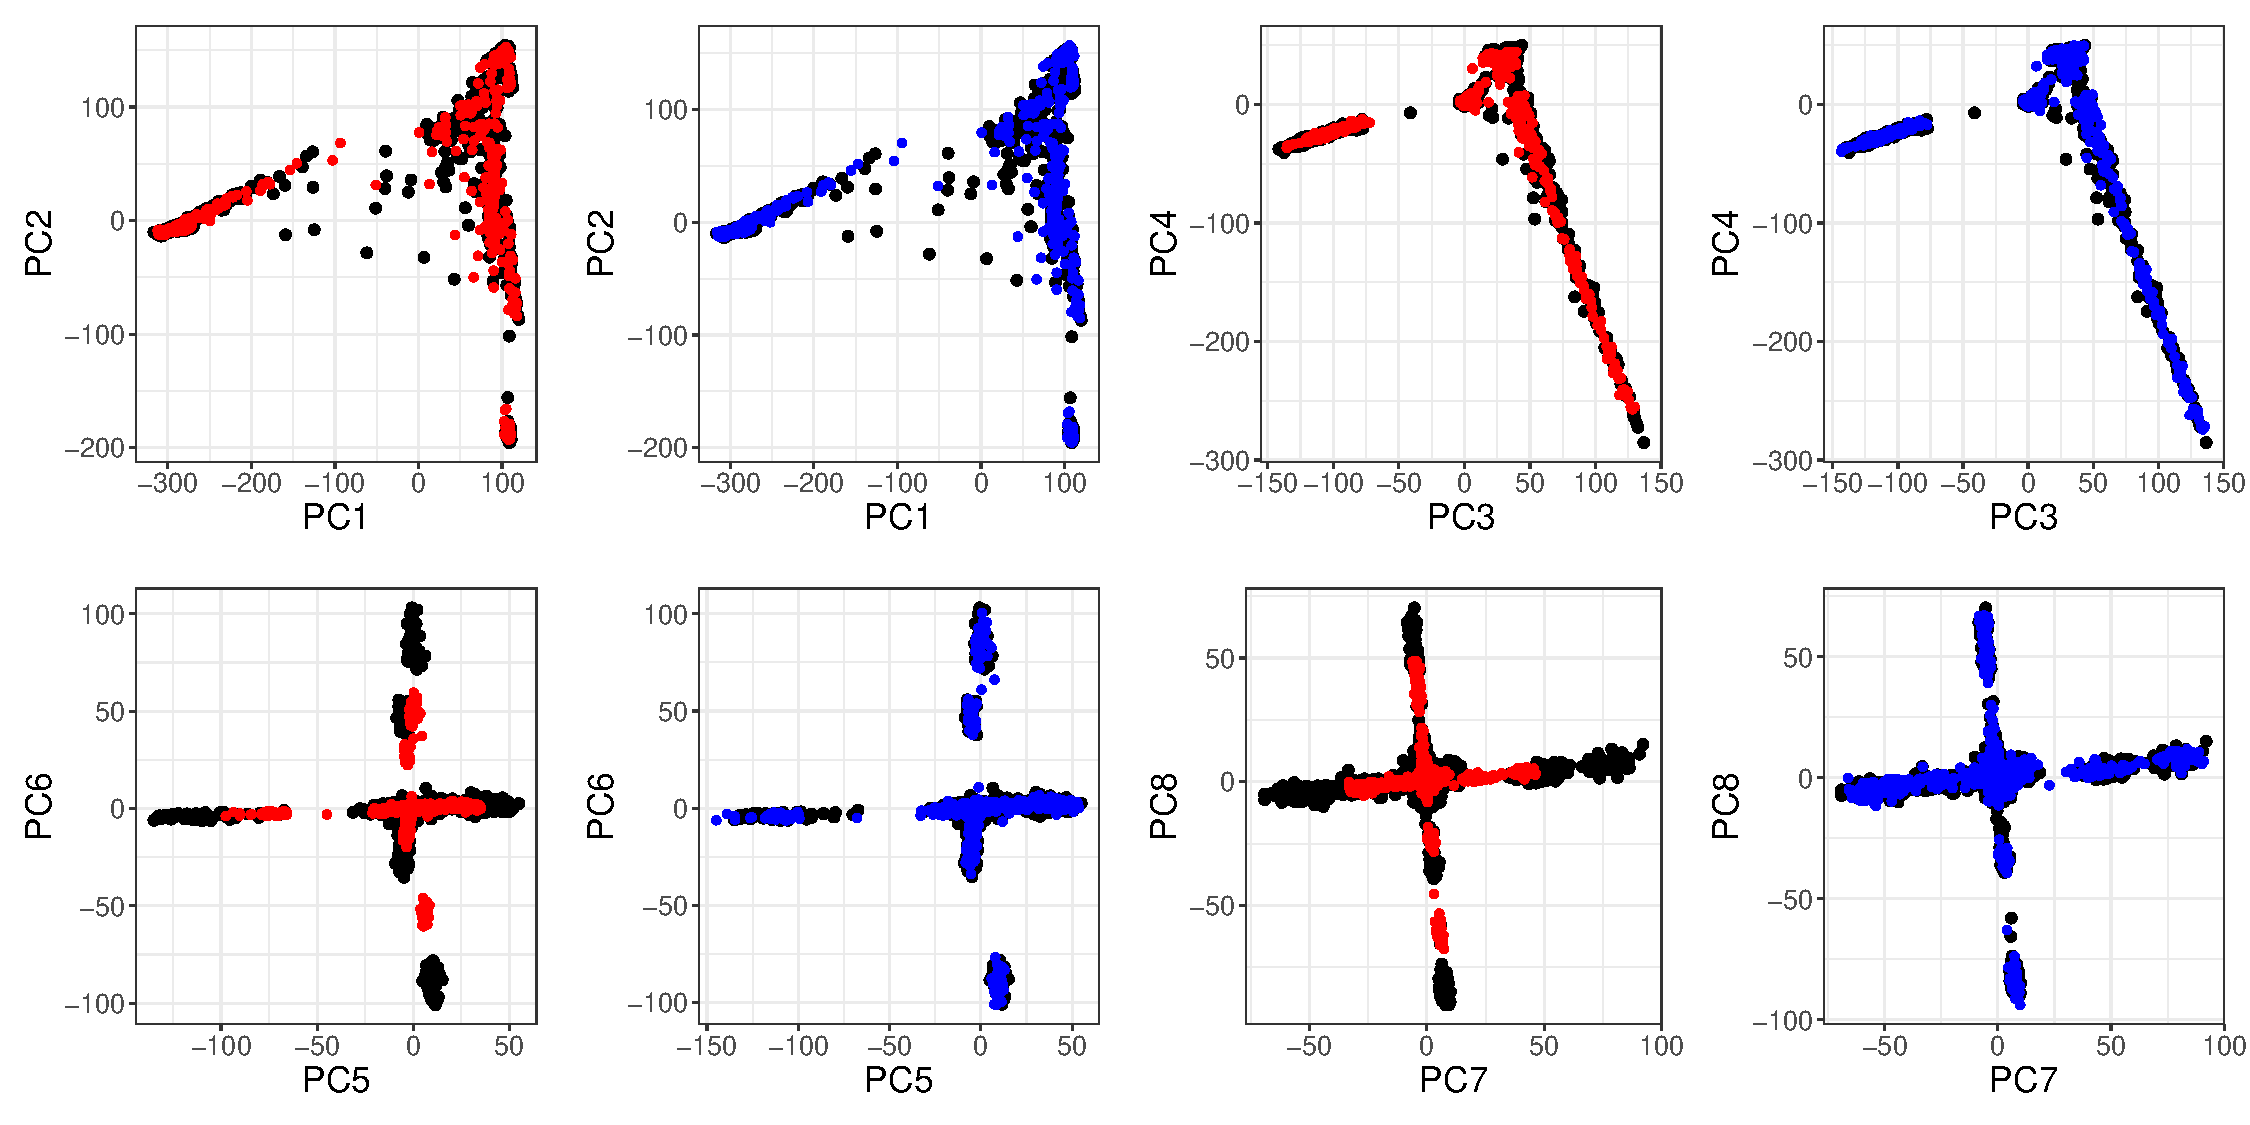
\includegraphics[width=0.8\textwidth]{proj1000G-PC1-8.pdf}}
\caption{Principal Component (PC) scores 1 to 8 of the 1000 Genomes project.
Black points are the 60\% individuals used for computing PCA.
Red points are the 40\% remaining individuals, projected by simply multiplying their genotypes by the corresponding PC loadings.
Blue points are the 40\% remaining individuals, projected using the Online Augmentation, Decomposition, and Procrustes (OADP) transformation.
\label{fig:proj1000G}}
\end{figure}


\subsection{PCA of the UK Biobank}

Principal Components (PC) loadings reported by the UK Biobank clearly show that PC19 to PC40 capture LD structure, which is also the case for PC16 and PC18, although less pronounced (see peaks in figure \ref{fig:UKBB-loadings40}). 
Moreover, our automatic procedure removing long-range LD regions did not converge after 5 iterations, meaning that it kept detecting long-range LD regions at each iteration. Therefore, we were able to capture only 16 PCs that shows population stratification and not LD structure (Figures \ref{fig:UKBB-screeplot}, \ref{fig:UKBB-scores} and \ref{fig:UKBB-loadings}).

Then, we computed again PCA after restricting the individuals included in the computations: we randomly subsampled UKBB data to use only 10,000 British individuals (out of 431,029) and 5000 Irish individuals (out of 12,755), while keeping all individuals with other self-reported individuals. 
We further removed all pairs of related individuals reported by the UKBB (both individuals in each pair). 
This resulted in 48,942 individuals that we used to compute 50 PCs, which took less than 3 hours using function \texttt{bed\_autoSVD} (that converged after 4 iterations of automatic LD removal). 
We show that we are able to capture at least 40 PCs that display visual population structure (Figures \ref{fig:UKBB-scores2} and \ref{fig:UKBB-screeplot2}).
We then projected all 439,429 remaining individuals from UKBB onto this PCA space in 41 minutes. Note that these individuals are not supposed to be related to any of the 48,942 individuals used for training PCA because we removed both individuals from each pair of related individuals in UKBB. Projection of new individuals show again clear shrinkage when using simple projection (between 1.00 for PC1 and 1.80 for PC50), but no visible bias when using OADP projection (Figure \ref{fig:projUKBB-related}).

\noindent[SHOW INITIAL PC SCORES OF UKBB?]

\noindent[COMPUTE MAHA ON LOADINGS TO SHOW THE PEAKS SUMMARIZED IN ALL 16-18 PCS?]

\noindent[SHOW THAT PROCEDURE IS OKAY FOR SMALLER DATASETS?]

\noindent[SHOW ABLE TO RECONSTRUCT PCA? MAYBE NOT PC17]


%%%%%%%%%%%%%%%%%%%%%%%%%%%%%%%%%%%%%%%%%%%%%%%%%%%%%%%%%%%%%%%%%%%%%%%%%%%%%%%%

\section{Discussion}

\noindent[LIMITATION 1: RUN MULTIPLE TIMES / FAIL TO SPEED UP]

\noindent[LIMITATION 2: FAIL TO PROJECT RELATED INDIVIDUALS WITH OADP -> RESTRICT MORE.]


\subsection{Conclusion}




%%%%%%%%%%%%%%%%%%%%%%%%%%%%%%%%%%%%%%%%%%%%%%%%%%%%%%%%%%%%%%%%%%%%%%%%%%%%%%%%

%\newpage

\section*{Acknowledgements}

Authors thank Rounak Dey and Seunggeun Lee for helpful discussions about PCA projection.
This research has been conducted using the UK Biobank Resource under Application Number 25589.

F.P., J.J.M.\ and B.J.V.\ acknowledge Niels Bohr Professorship from the Danish National Research Foundation to Prof.\ John J.\ McGrath, and the Lundbeck Foundation Initiative for Integrative Psychiatric Research, iPSYCH (R248-2017-2003).

\section*{Declaraction of Interests}

Michael Blum is an employee of OWKIN France.
The other authors declare no competing interests.

%%%%%%%%%%%%%%%%%%%%%%%%%%%%%%%%%%%%%%%%%%%%%%%%%%%%%%%%%%%%%%%%%%%%%%%%%%%%%%%%

%\newpage

\bibliographystyle{natbib}
\bibliography{refs}

%%%%%%%%%%%%%%%%%%%%%%%%%%%%%%%%%%%%%%%%%%%%%%%%%%%%%%%%%%%%%%%%%%%%%%%%%%%%%%%%

\newpage
\section*{Supplementary Materials}

\renewcommand{\thefigure}{S\arabic{figure}}
\setcounter{figure}{0}
\renewcommand{\thetable}{S\arabic{table}}
\setcounter{table}{0}

\subsection*{Optimised OADP transformation}

We implement an optimised version of the Online Augmentation, Decomposition, and Procrustes (OADP) transformation when using $K''=K'=K$ \cite[]{zhang2019fast}.
We assume that the $K$-partial Singular Value Decomposition (SVD) of the reference matrix $X$ (of size $n \times p$) has been computed as $U \Delta V^T$. There are several steps to perform OADP transformation for each sample $y$ (of size $1 \times p$) of target matrix $Y$ (of size $m \times p$):
\begin{enumerate}
\item Calculate $l = y \cdot V$ (of size $1 \times K$), where $V$ are the K PC loadings. And $g = y \cdot h^T$ (of size $1 \times 1$), where $h = (y - l \cdot V^T) / ||y - l \cdot V^T||_2$. Actually, $||y - l \cdot V^T||_2^2 = y \cdot y^T - 2 \cdot y \cdot V \cdot l^T  + l \cdot V^T \cdot V \cdot l^T = y \cdot y^T - l \cdot l^T$ and $y \cdot (y - l \cdot V^T)^T = y \cdot y^T - y \cdot V \cdot l^T = y \cdot y^T - l \cdot l^T$. Then $g = \sqrt{y \cdot y^T - l \cdot l^T}$.
\item Calculate $Q^T Q$ where $$Q = \begin{bmatrix} \Delta & l^T \\ 0 & g \end{bmatrix}$$ so that $$Q^TQ = \begin{bmatrix} \Delta^2 & \Delta \cdot l^T \\ l \cdot \Delta & g^2 + l \cdot l^T \end{bmatrix} = \begin{bmatrix} \Delta^2 & \Delta \cdot l^T \\ l \cdot \Delta & y \cdot y^T \end{bmatrix}.$$ Note that we do not actually need to compute $g$, and that we can update the last row and column of $Q^T Q$ instead of computing it from an updated version of $Q$.
\item Get the eigen decomposition $Q^T Q = V' {\Delta'}^2 {V'}^T$ (truncated to $K$ components out of the $K+1$). Let us denote $V_2 = V' {\Delta'}$.
\item Calculate $$\begin{bmatrix} \widetilde{U} \\ \widetilde{u}  \end{bmatrix} = \begin{bmatrix} U & 0 \\ 0 & 1 \end{bmatrix} V_2 = \begin{bmatrix} U V_2[1{:}K,~] \\ V_2[K{+}1,~] \end{bmatrix} $$
\item Find the Procrustes transformation from $\widetilde{U}$ to $U \Delta$. As $\widetilde{U}$ and $U \Delta$ have both their columns centered already (since $U$ does), the Procrustes transformation $\rho \widetilde{U} A$, where $\rho$ is a scaling coefficient and $A$ is an orthonomal projection matrix that minimise the Frobenius norm of $(\rho \widetilde{U} A - U)$, is given by $A = V'' {U''}^T$ and $\rho = \frac{\text{trace}(\Delta'')}{\text{trace}(\widetilde{U}^T \widetilde{U})}$ where $U'' \Delta'' {V''}^T$ is the full SVD of $(U \Delta)^T \widetilde{U}$ \cite[]{wang2015improved}. 
As $U^T U = I$, we note that $(U \Delta)^T \widetilde{U} = \Delta V_2[1{:}K,~]$ and that $\rho = \frac{\text{trace}(\Delta'')}{\text{trace}({V_2[1{:}K,~]}^T V_2[1{:}K,~])}$, therefore we do not need to explicitly compute $\widetilde{U}$. 
\item Apply the previous transformation to $\widetilde{u}$ to get the projection of $y$ in the reference PCA space (i.e.\ $\rho \widetilde{u} A$).
\end{enumerate}


%%%%%%%%%%%%%%%%%%%%%%%%%%%%%%%%%%%%%%%%%%%%%%%%%%%%%%%%%%%%%%%%%%%%%%%%%%%%%%%%

\clearpage

\subsection*{Supplementary figures}

%%%%%%%%%%%%%%%%%%%%%%%%%%%%%%%%%%%%%%%%%%%%%%%%%%%%%%%%%%%%%%%%%%%%%%%%%%%%%%%%

\vspace*{1em}

\begin{figure}[!htpb]
\centerline{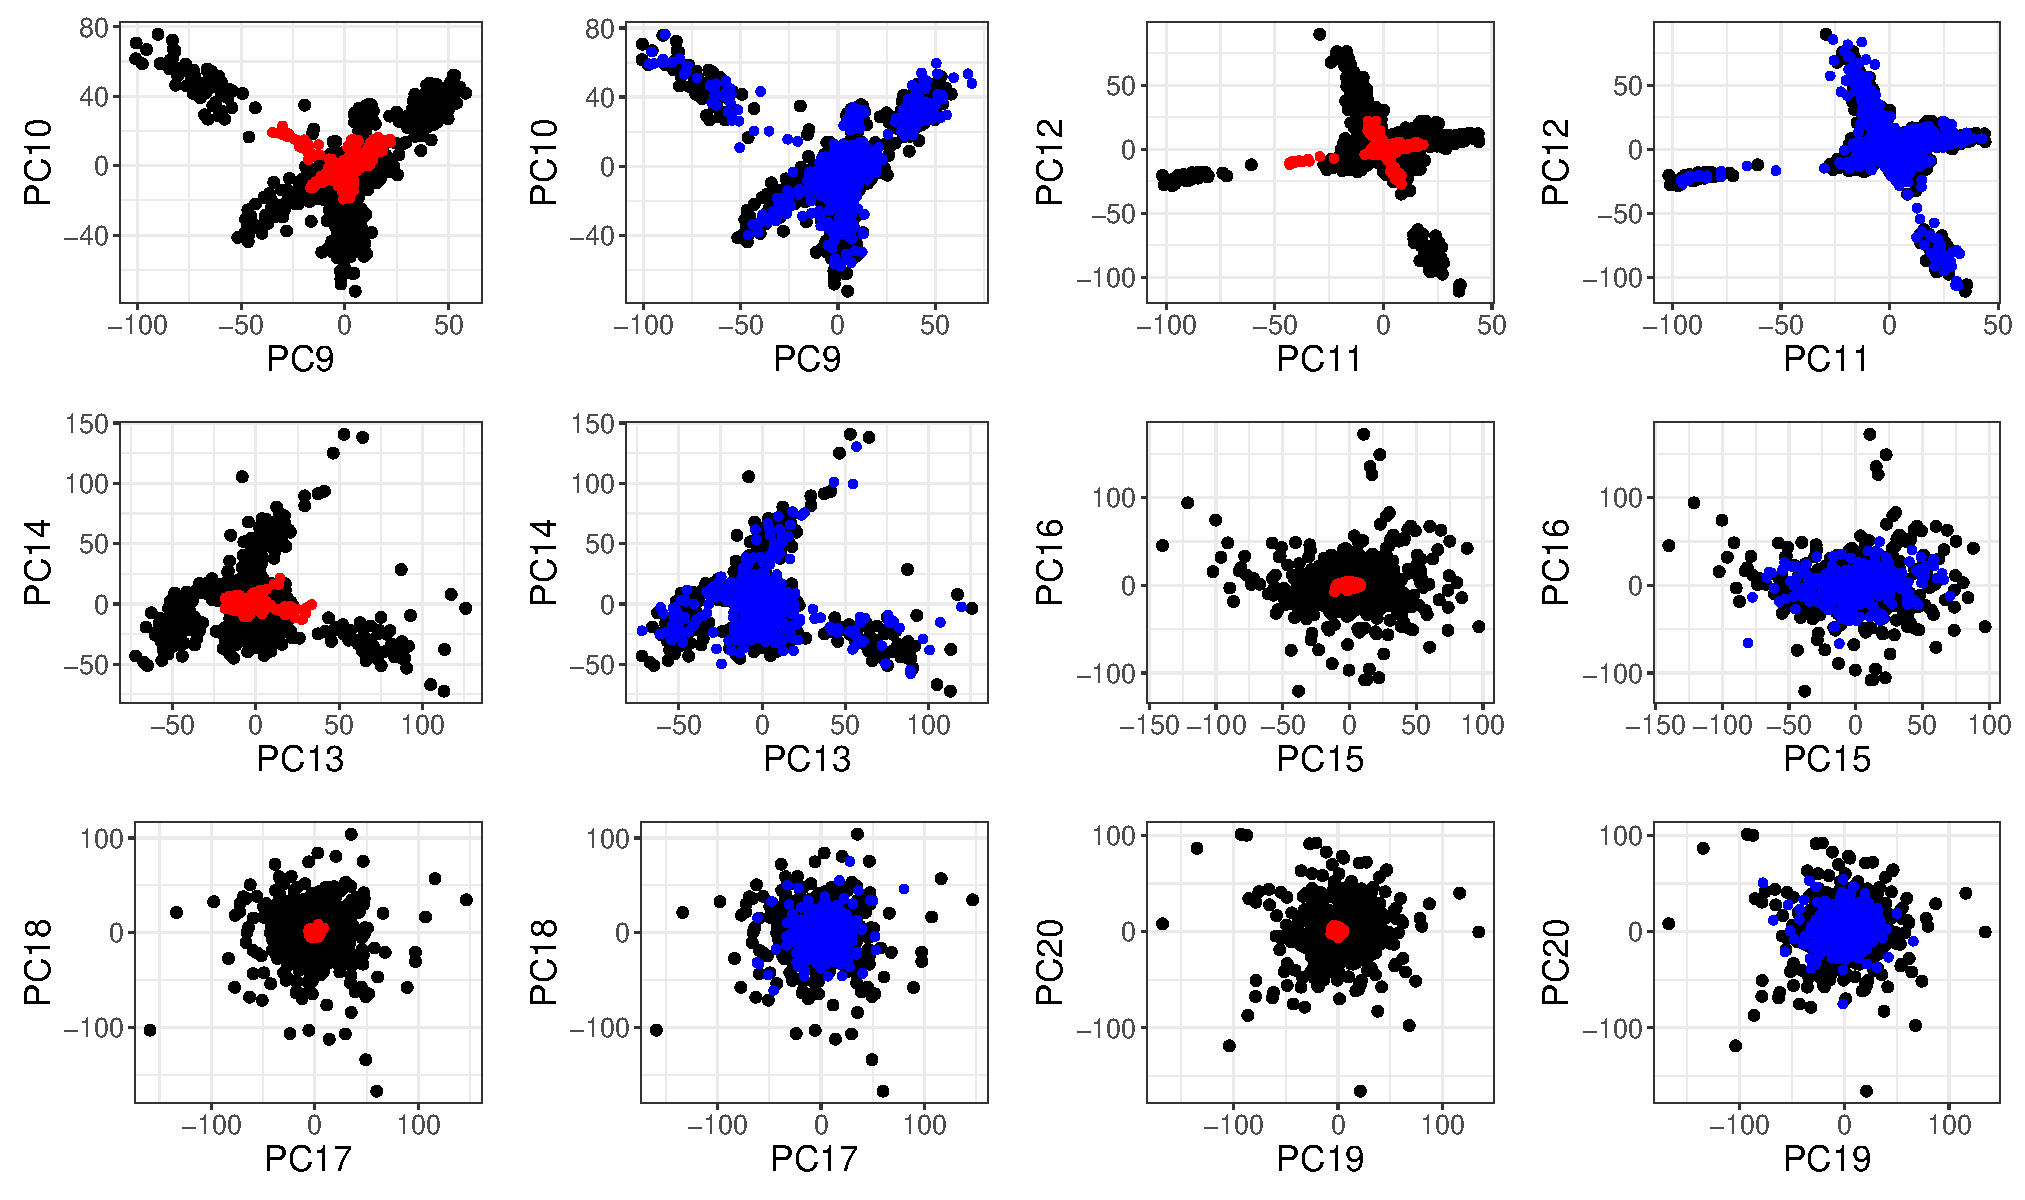
\includegraphics[width=0.9\textwidth]{proj1000G-PC9-20.pdf}}
\caption{Principal Component (PC) scores 9 to 20 of the 1000 Genomes project.
Black points are the 60\% individuals used for computing PCA.
Red points are the 40\% remaining individuals, projected by simply multiplying their genotypes by the corresponding PC loadings.
Blue points are the 40\% remaining individuals, projected using the Online Augmentation, Decomposition, and Procrustes (OADP) transformation.
\label{fig:proj1000G-2}}
\end{figure}

\vspace*{1em}

\begin{figure}[!htpb]
\centerline{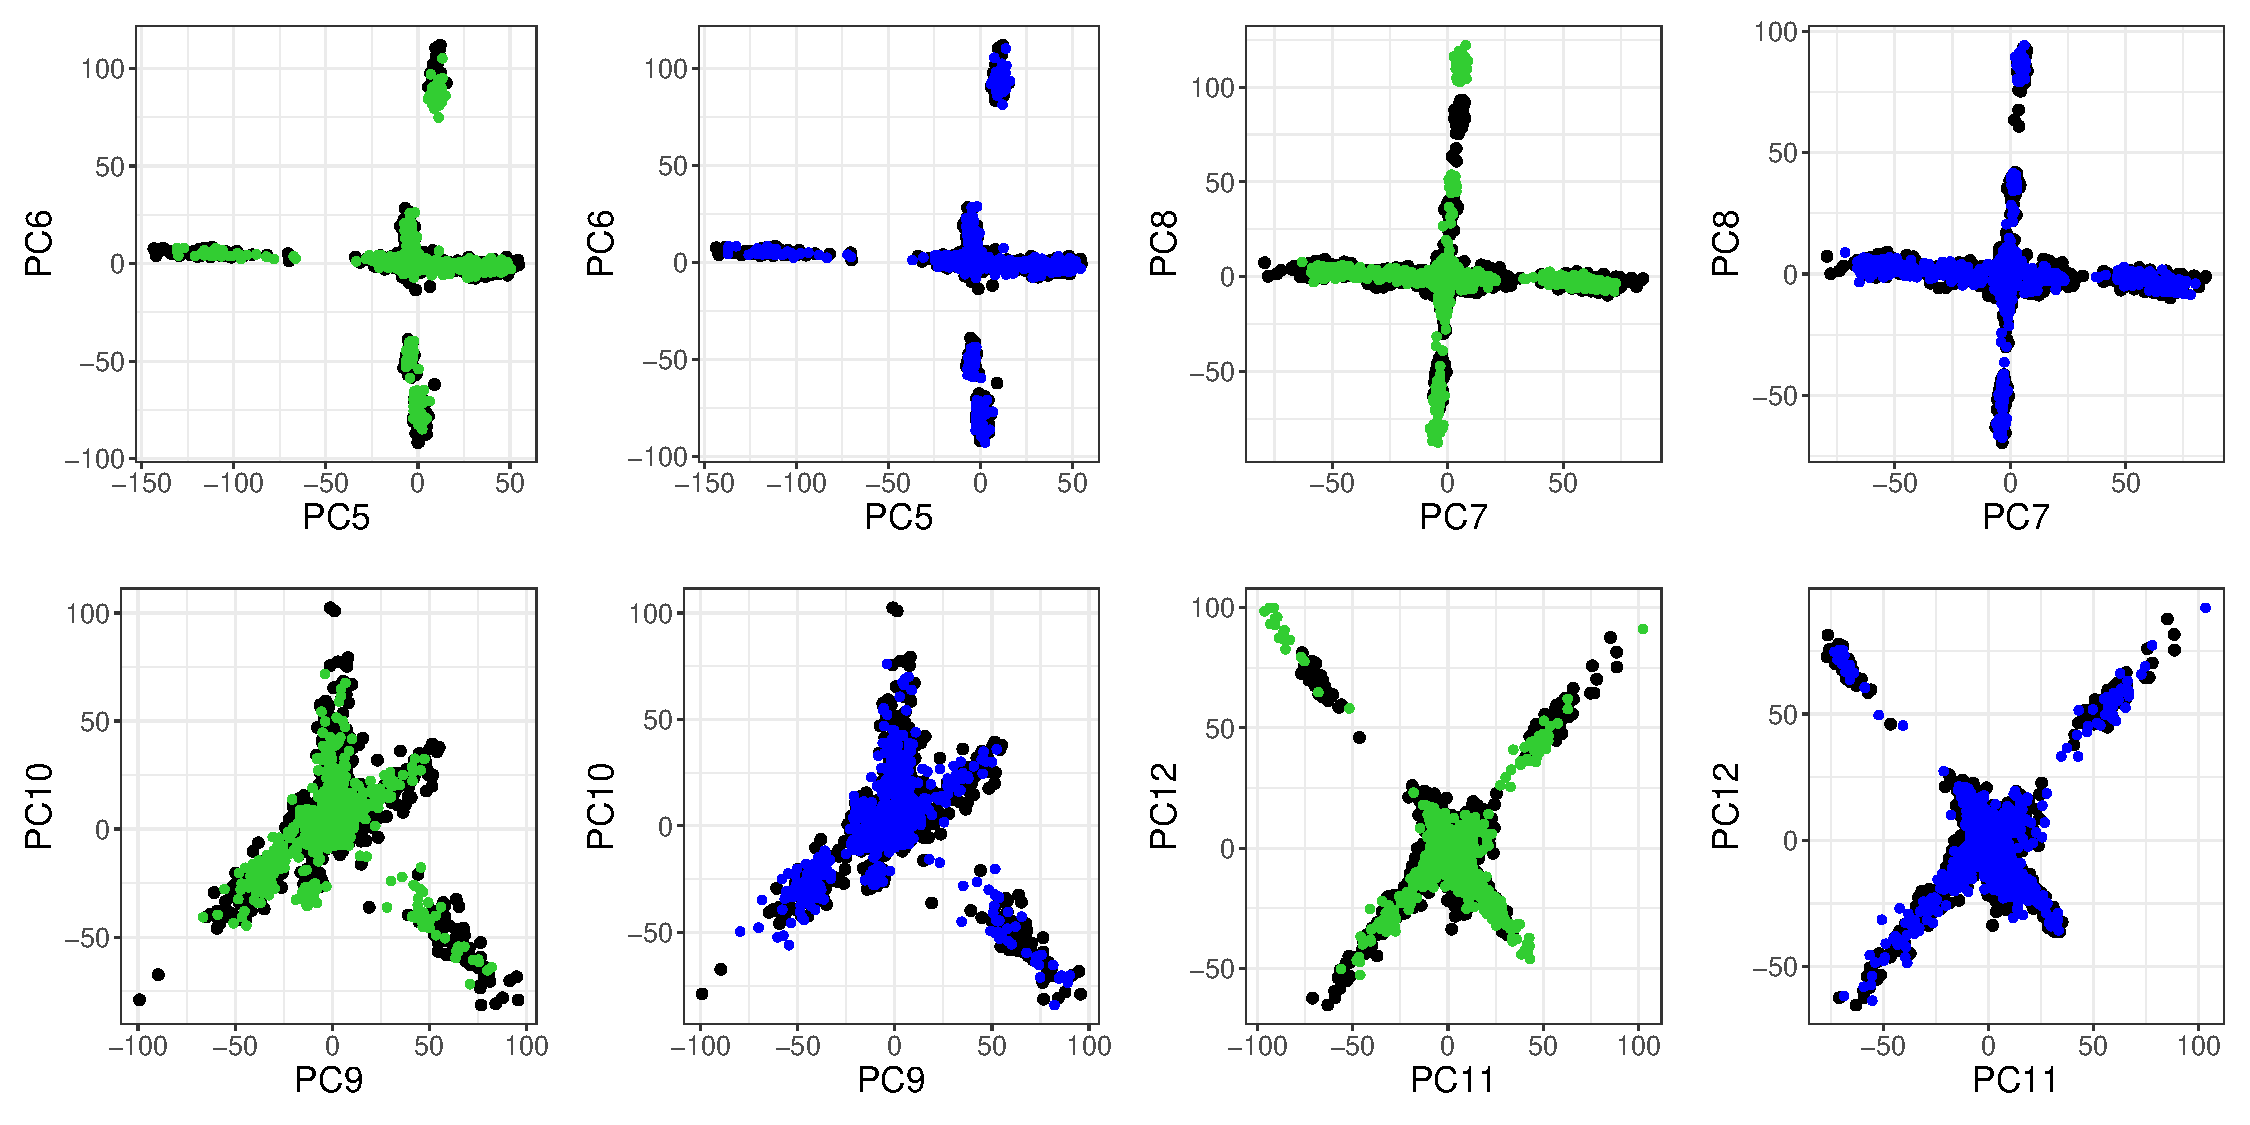
\includegraphics[width=0.9\textwidth]{proj1000G-PC5-12.pdf}}
\caption{Principal Component (PC) scores 5 to 12 of the 1000 Genomes project.
Black points are the 60\% individuals used for computing PCA.
Green points are the 40\% remaining individuals, projected by multiplying their genotypes by the corresponding PC loadings, further corrected using theoritical asymptotic shrinkage factors.
Blue points are the 40\% remaining individuals, projected using the Online Augmentation, Decomposition, and Procrustes (OADP) transformation.
\label{fig:proj1000G-3}}
\end{figure}

\begin{figure}[!htpb]
\centerline{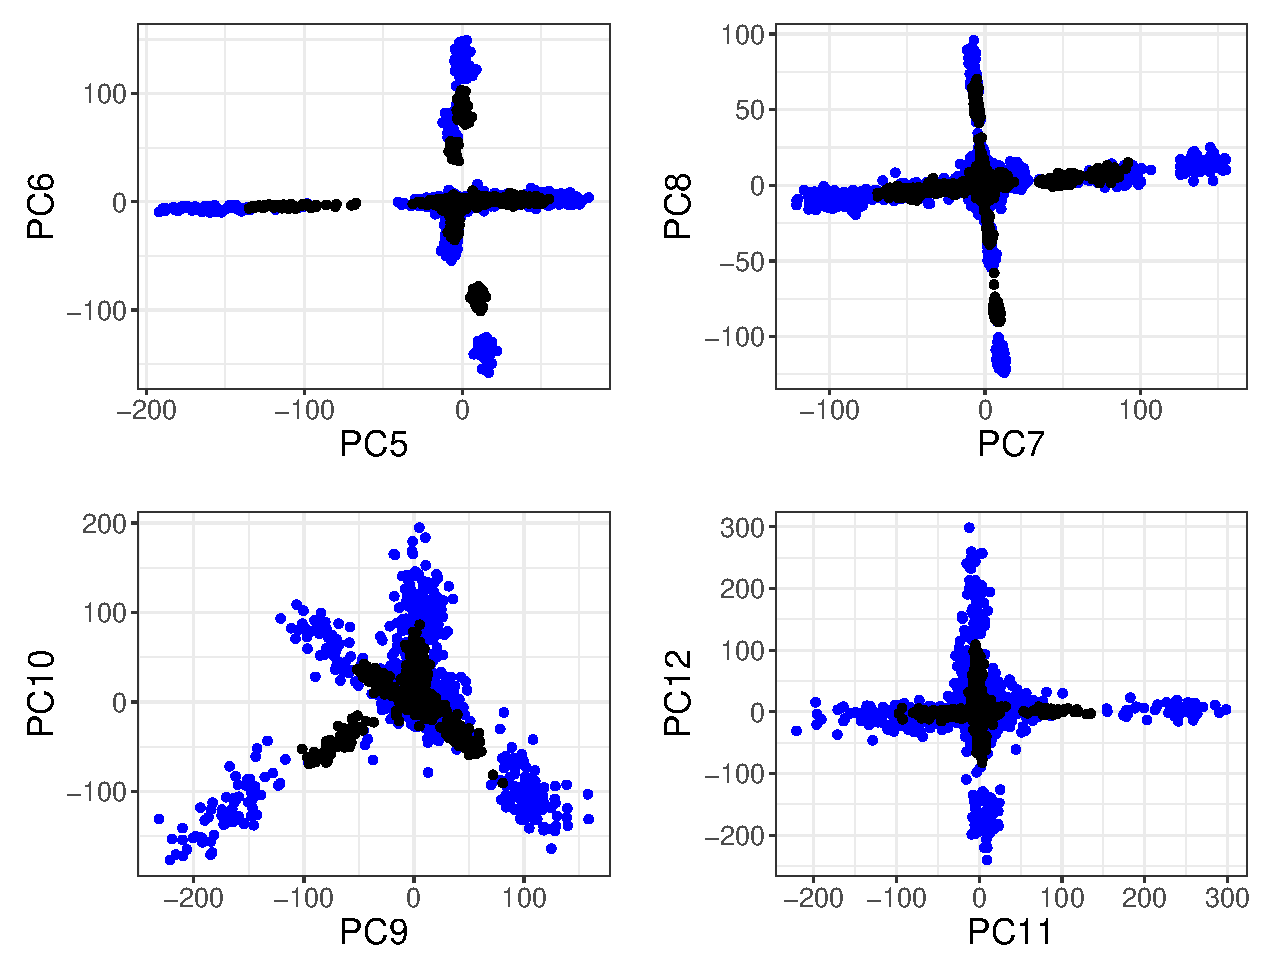
\includegraphics[width=0.9\textwidth]{proj1000G-related.pdf}}
\caption{Principal Component (PC) scores 5 to 12 of the 1000 Genomes project.
Black points are the 60\% individuals used for computing PCA.
Blue points are the same 60\% individuals, projected using the Online Augmentation, Decomposition, and Procrustes (OADP) transformation.
\label{fig:proj1000G-4}}
\end{figure}

\begin{figure}[!htpb]
\centerline{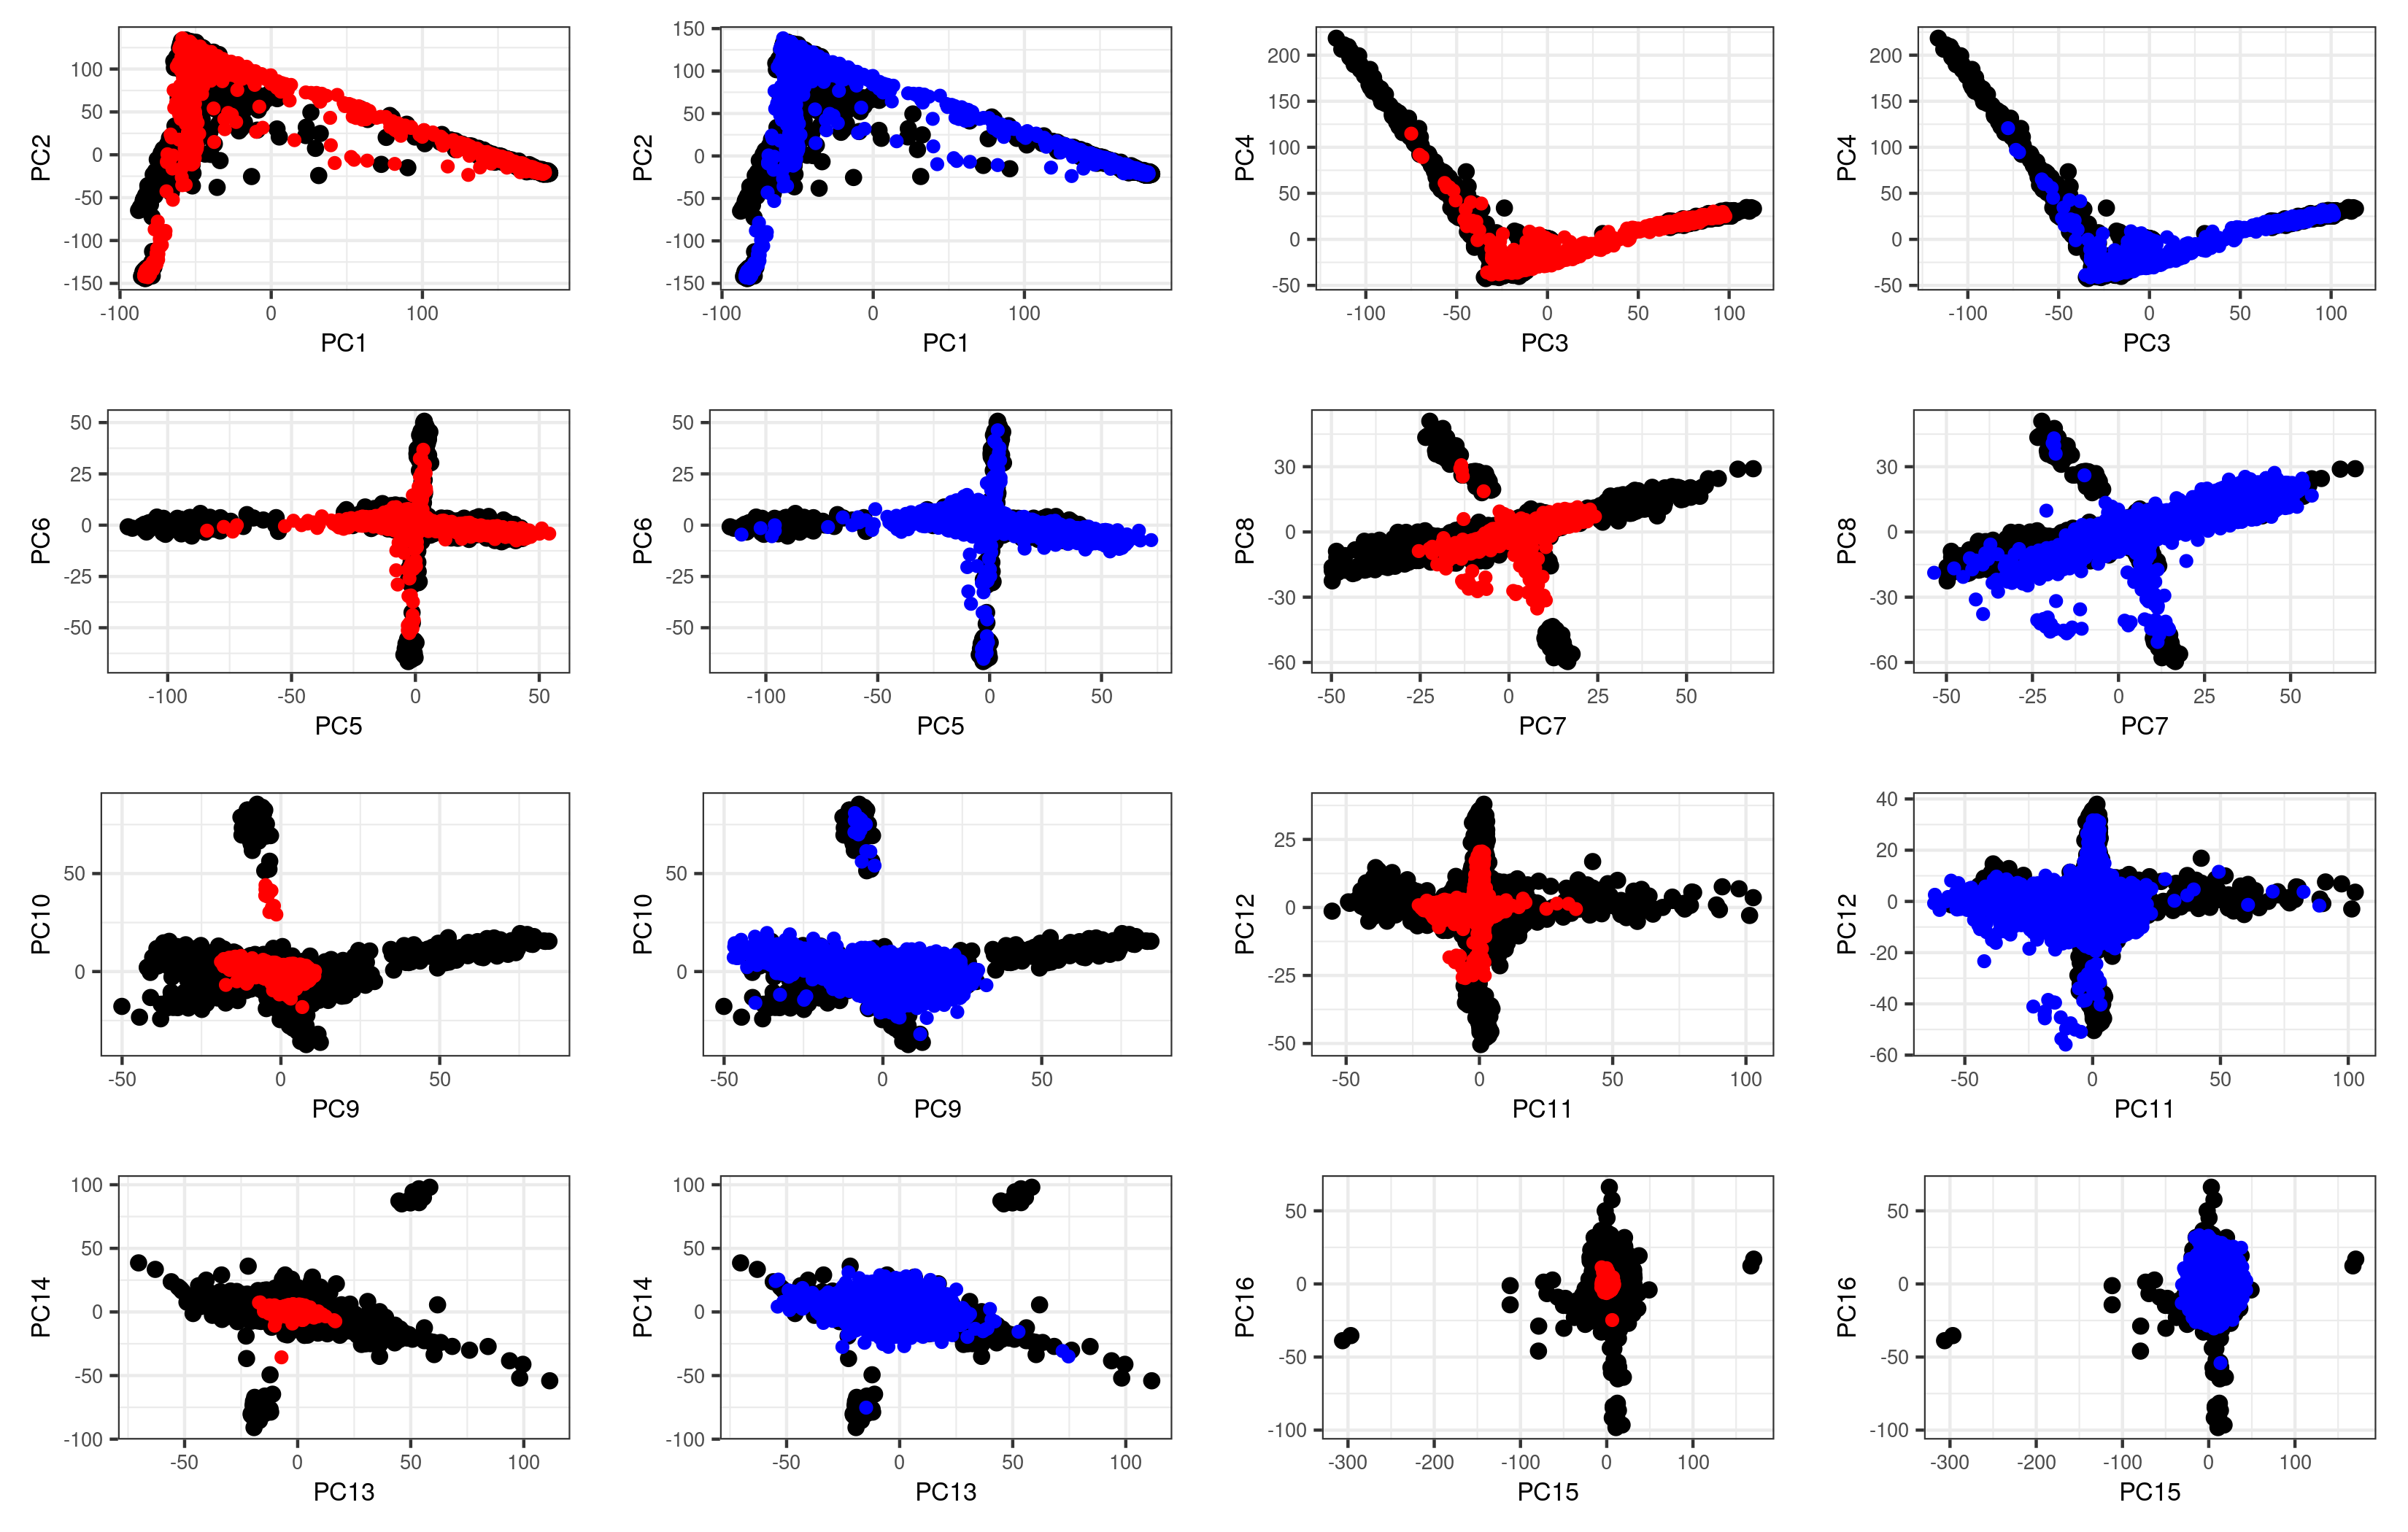
\includegraphics[width=0.9\textwidth]{proj1000G-UKBB.png}}
\caption{Principal Component (PC) scores 1 to 16 of the 1000 Genomes project and projected individuals from the UK Biobank.
Black points are PC scores of 1000G individuals used for computing PCA.
Blue points are the 488,371 individuals from the UK Biobank, projected using the Online Augmentation, Decomposition, and Procrustes (OADP) transformation. 
Note that only 20,000 random projected individuals are represented in this plot.
\label{fig:proj1000G-5}}
\end{figure}

\begin{figure}[!htpb]
\centerline{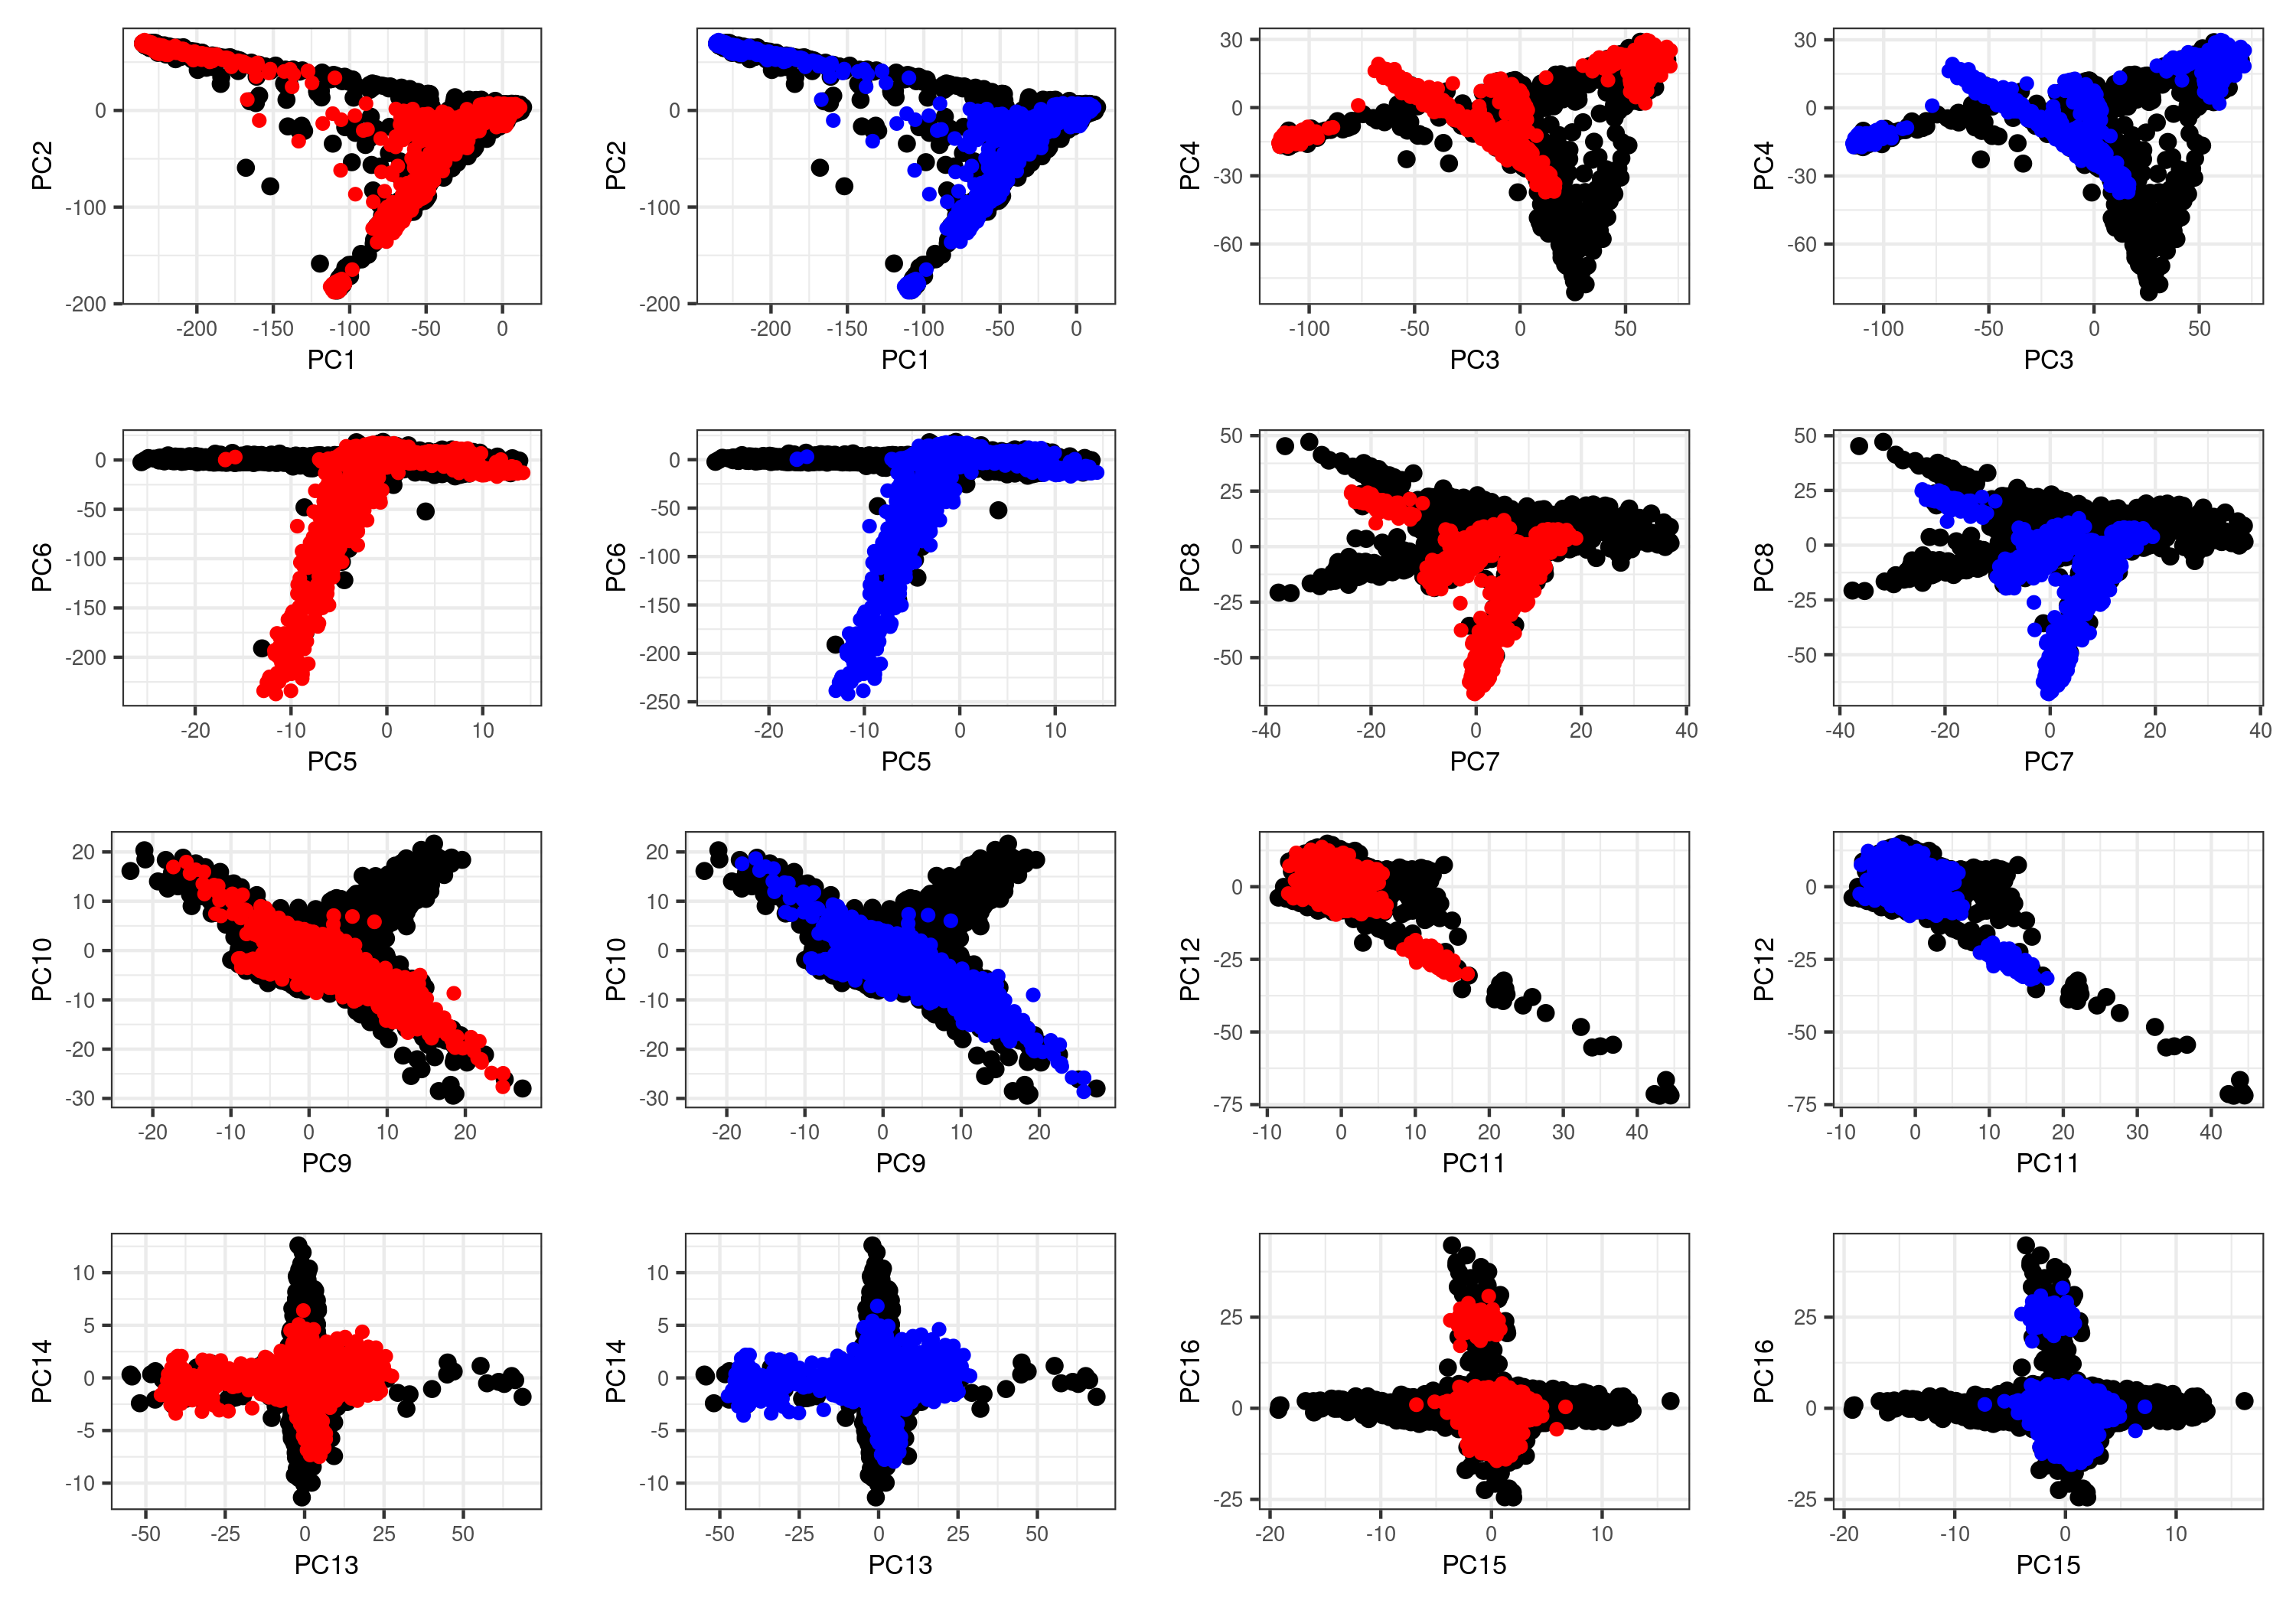
\includegraphics[width=0.8\textwidth]{proj1000G-UKBB2.png}}
\caption{Principal Component (PC) scores 1 to 16 from the UK Biobank and projected individuals of the 1000 Genomes (1000G) project.
Black points are the UK Biobank individuals used for computing PCA.
Red points are the individuals from 1000G, projected by simply multiplying their genotypes by the corresponding PC loadings.
Blue points are the individuals from 1000G, projected using the Online Augmentation, Decomposition, and Procrustes (OADP) transformation.
\label{fig:proj1000G-6}}
\end{figure}

%%%%%%%%%%%%%%%%%%%%%%%%%%%%%%%%%%%%%%%%%%%%%%%%%%%%%%%%%%%%%%%%%%%%%%%%%%%%%%%%

\begin{figure}[!htpb]
\centerline{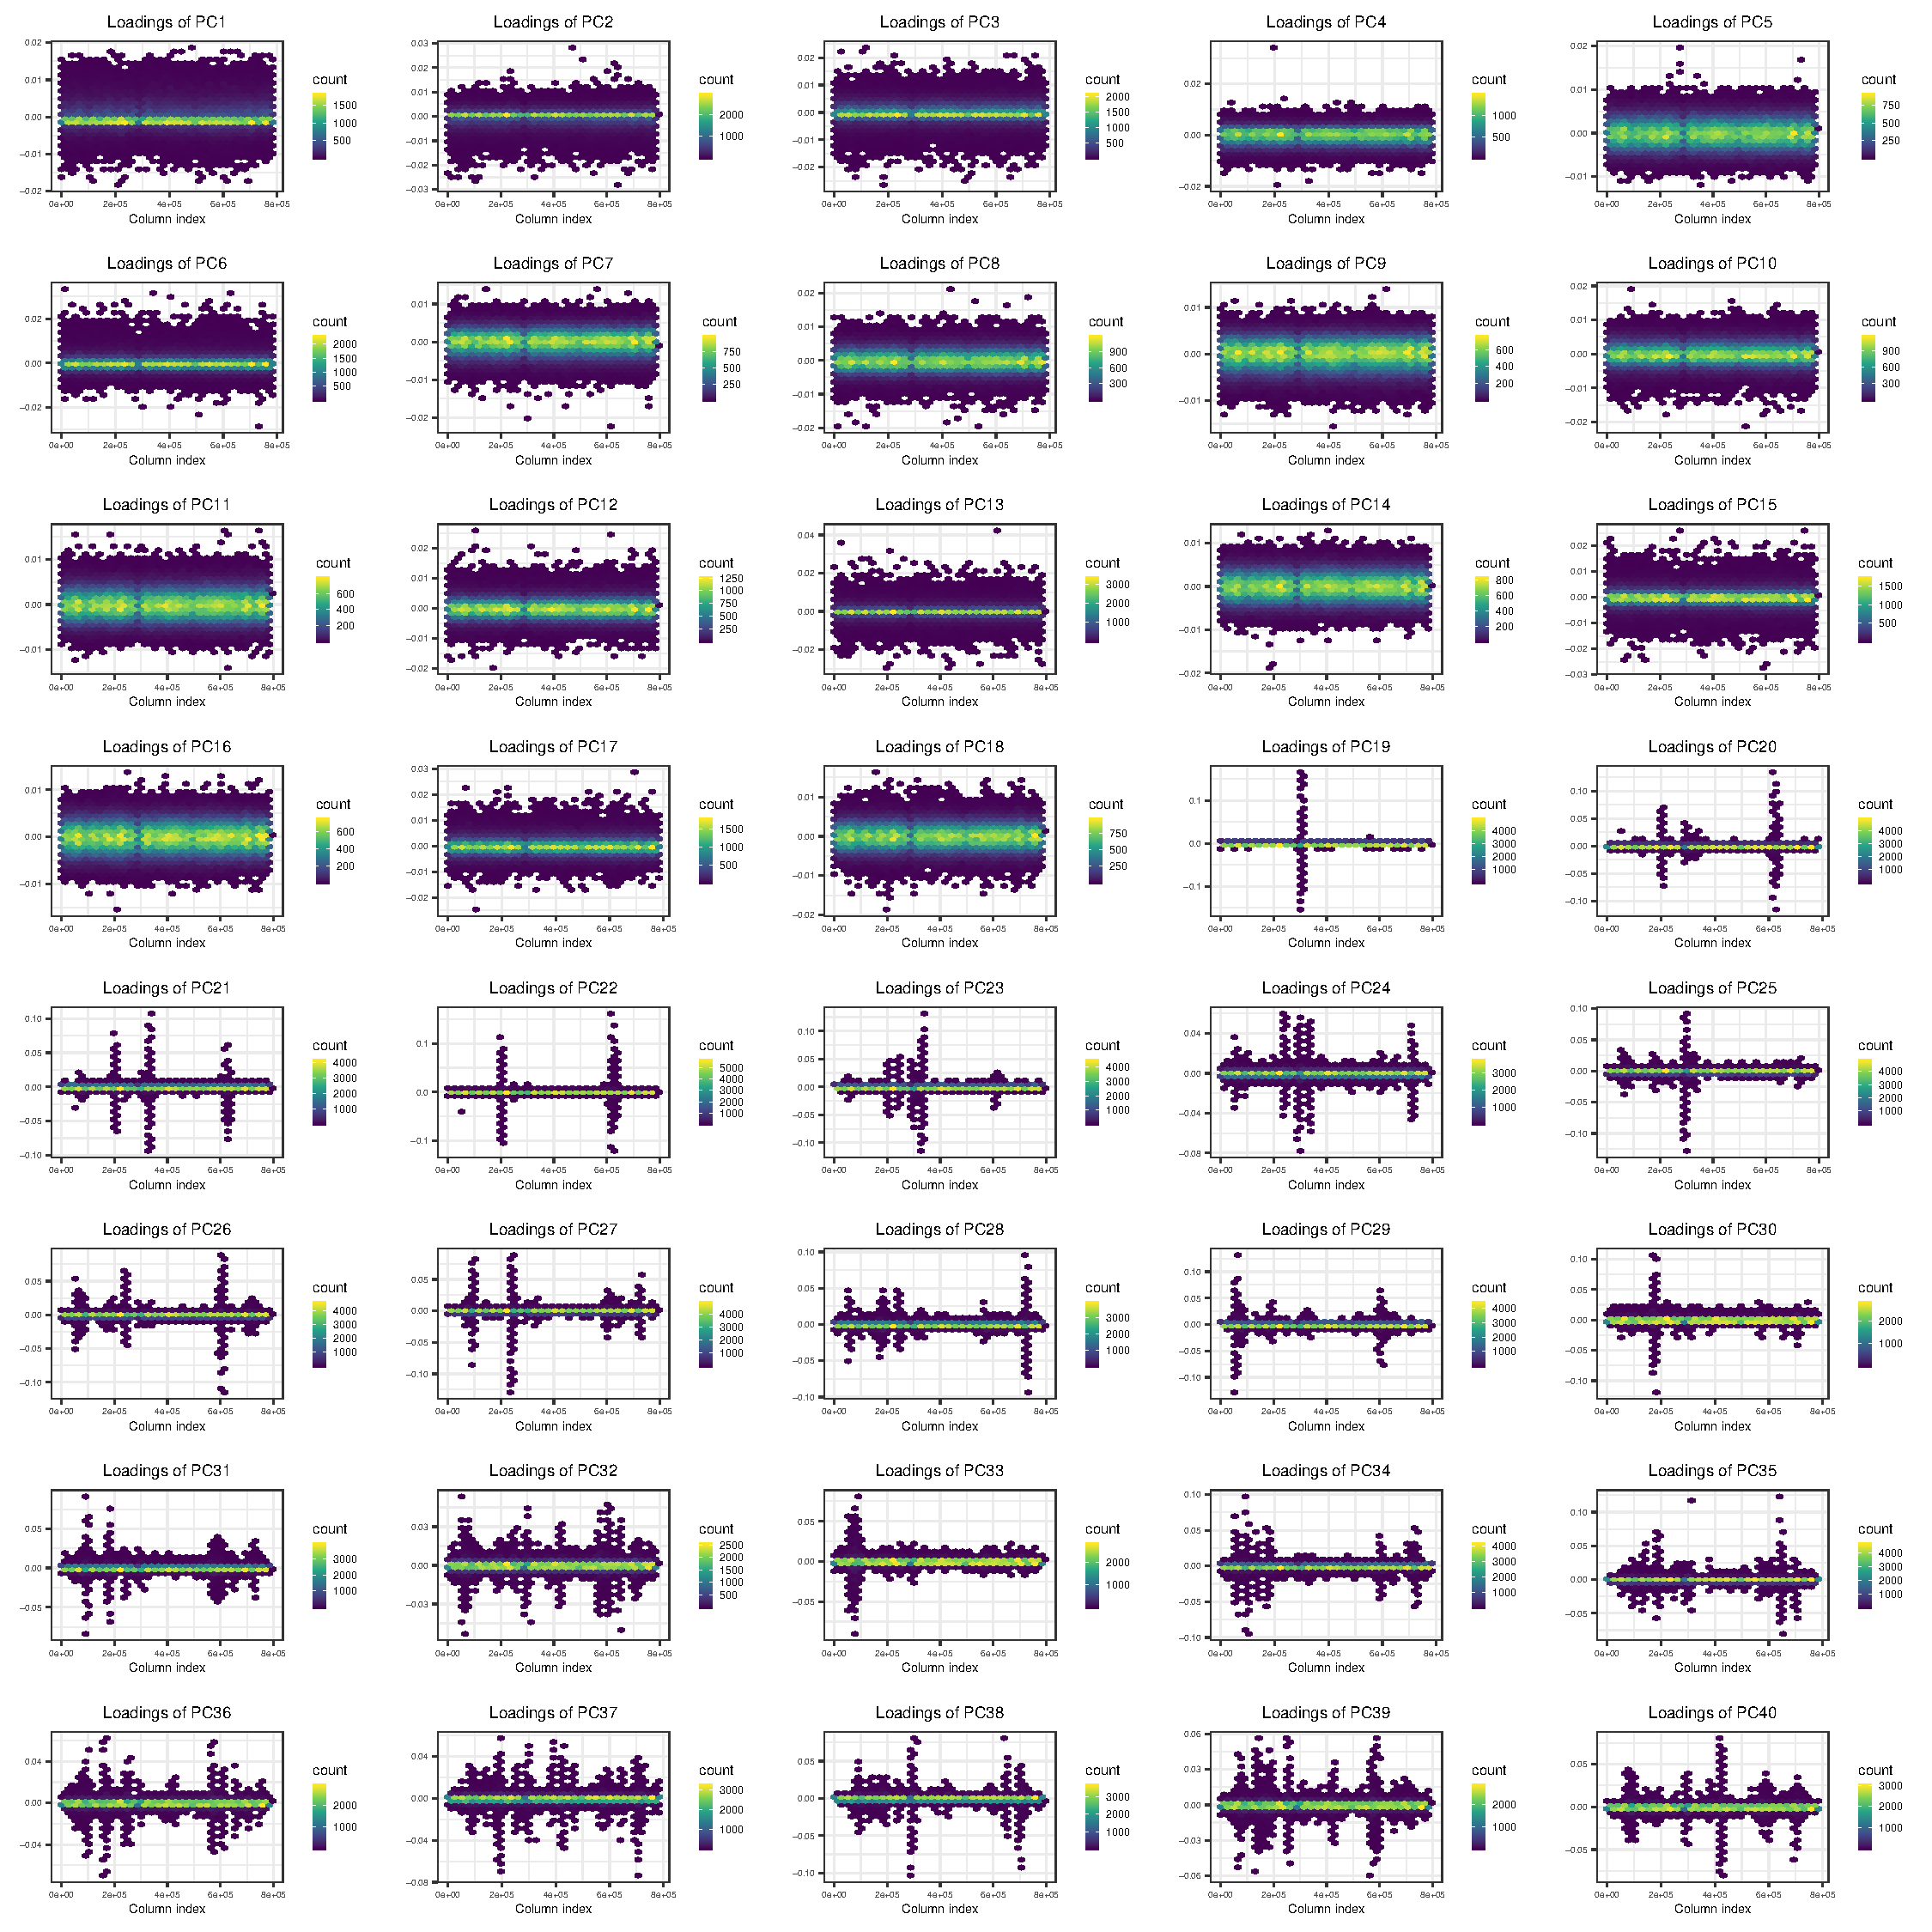
\includegraphics[width=0.9\textwidth]{UKBB-loadings1-40.pdf}}
\caption{Principal Component (PC) loadings 1 to 40 reported by the UK Biobank.
\label{fig:UKBB-loadings40}}
\end{figure}

\begin{figure}[!htpb]
\centerline{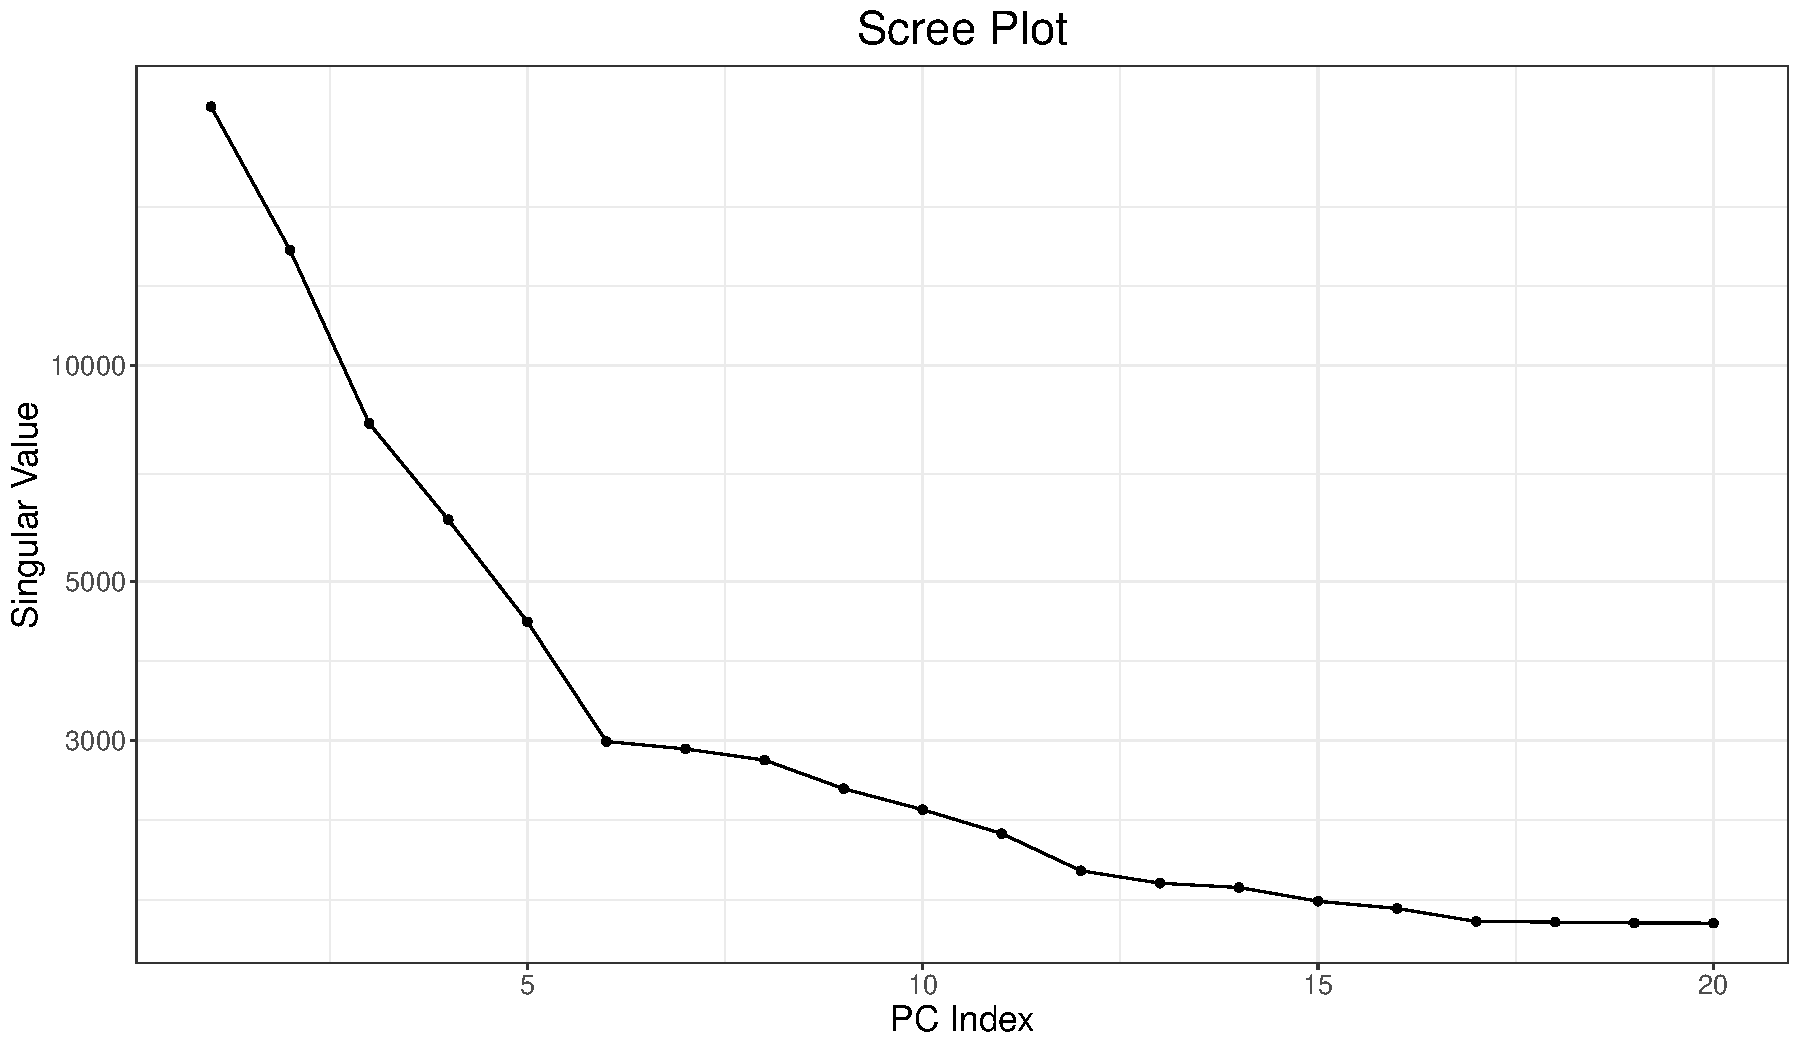
\includegraphics[width=0.8\textwidth]{UKBB-screeplot.pdf}}
\caption{Scree plot: plot of singular values computed from the UK Biobank.
\label{fig:UKBB-screeplot}}
\end{figure}

\begin{figure}[!htpb]
\centerline{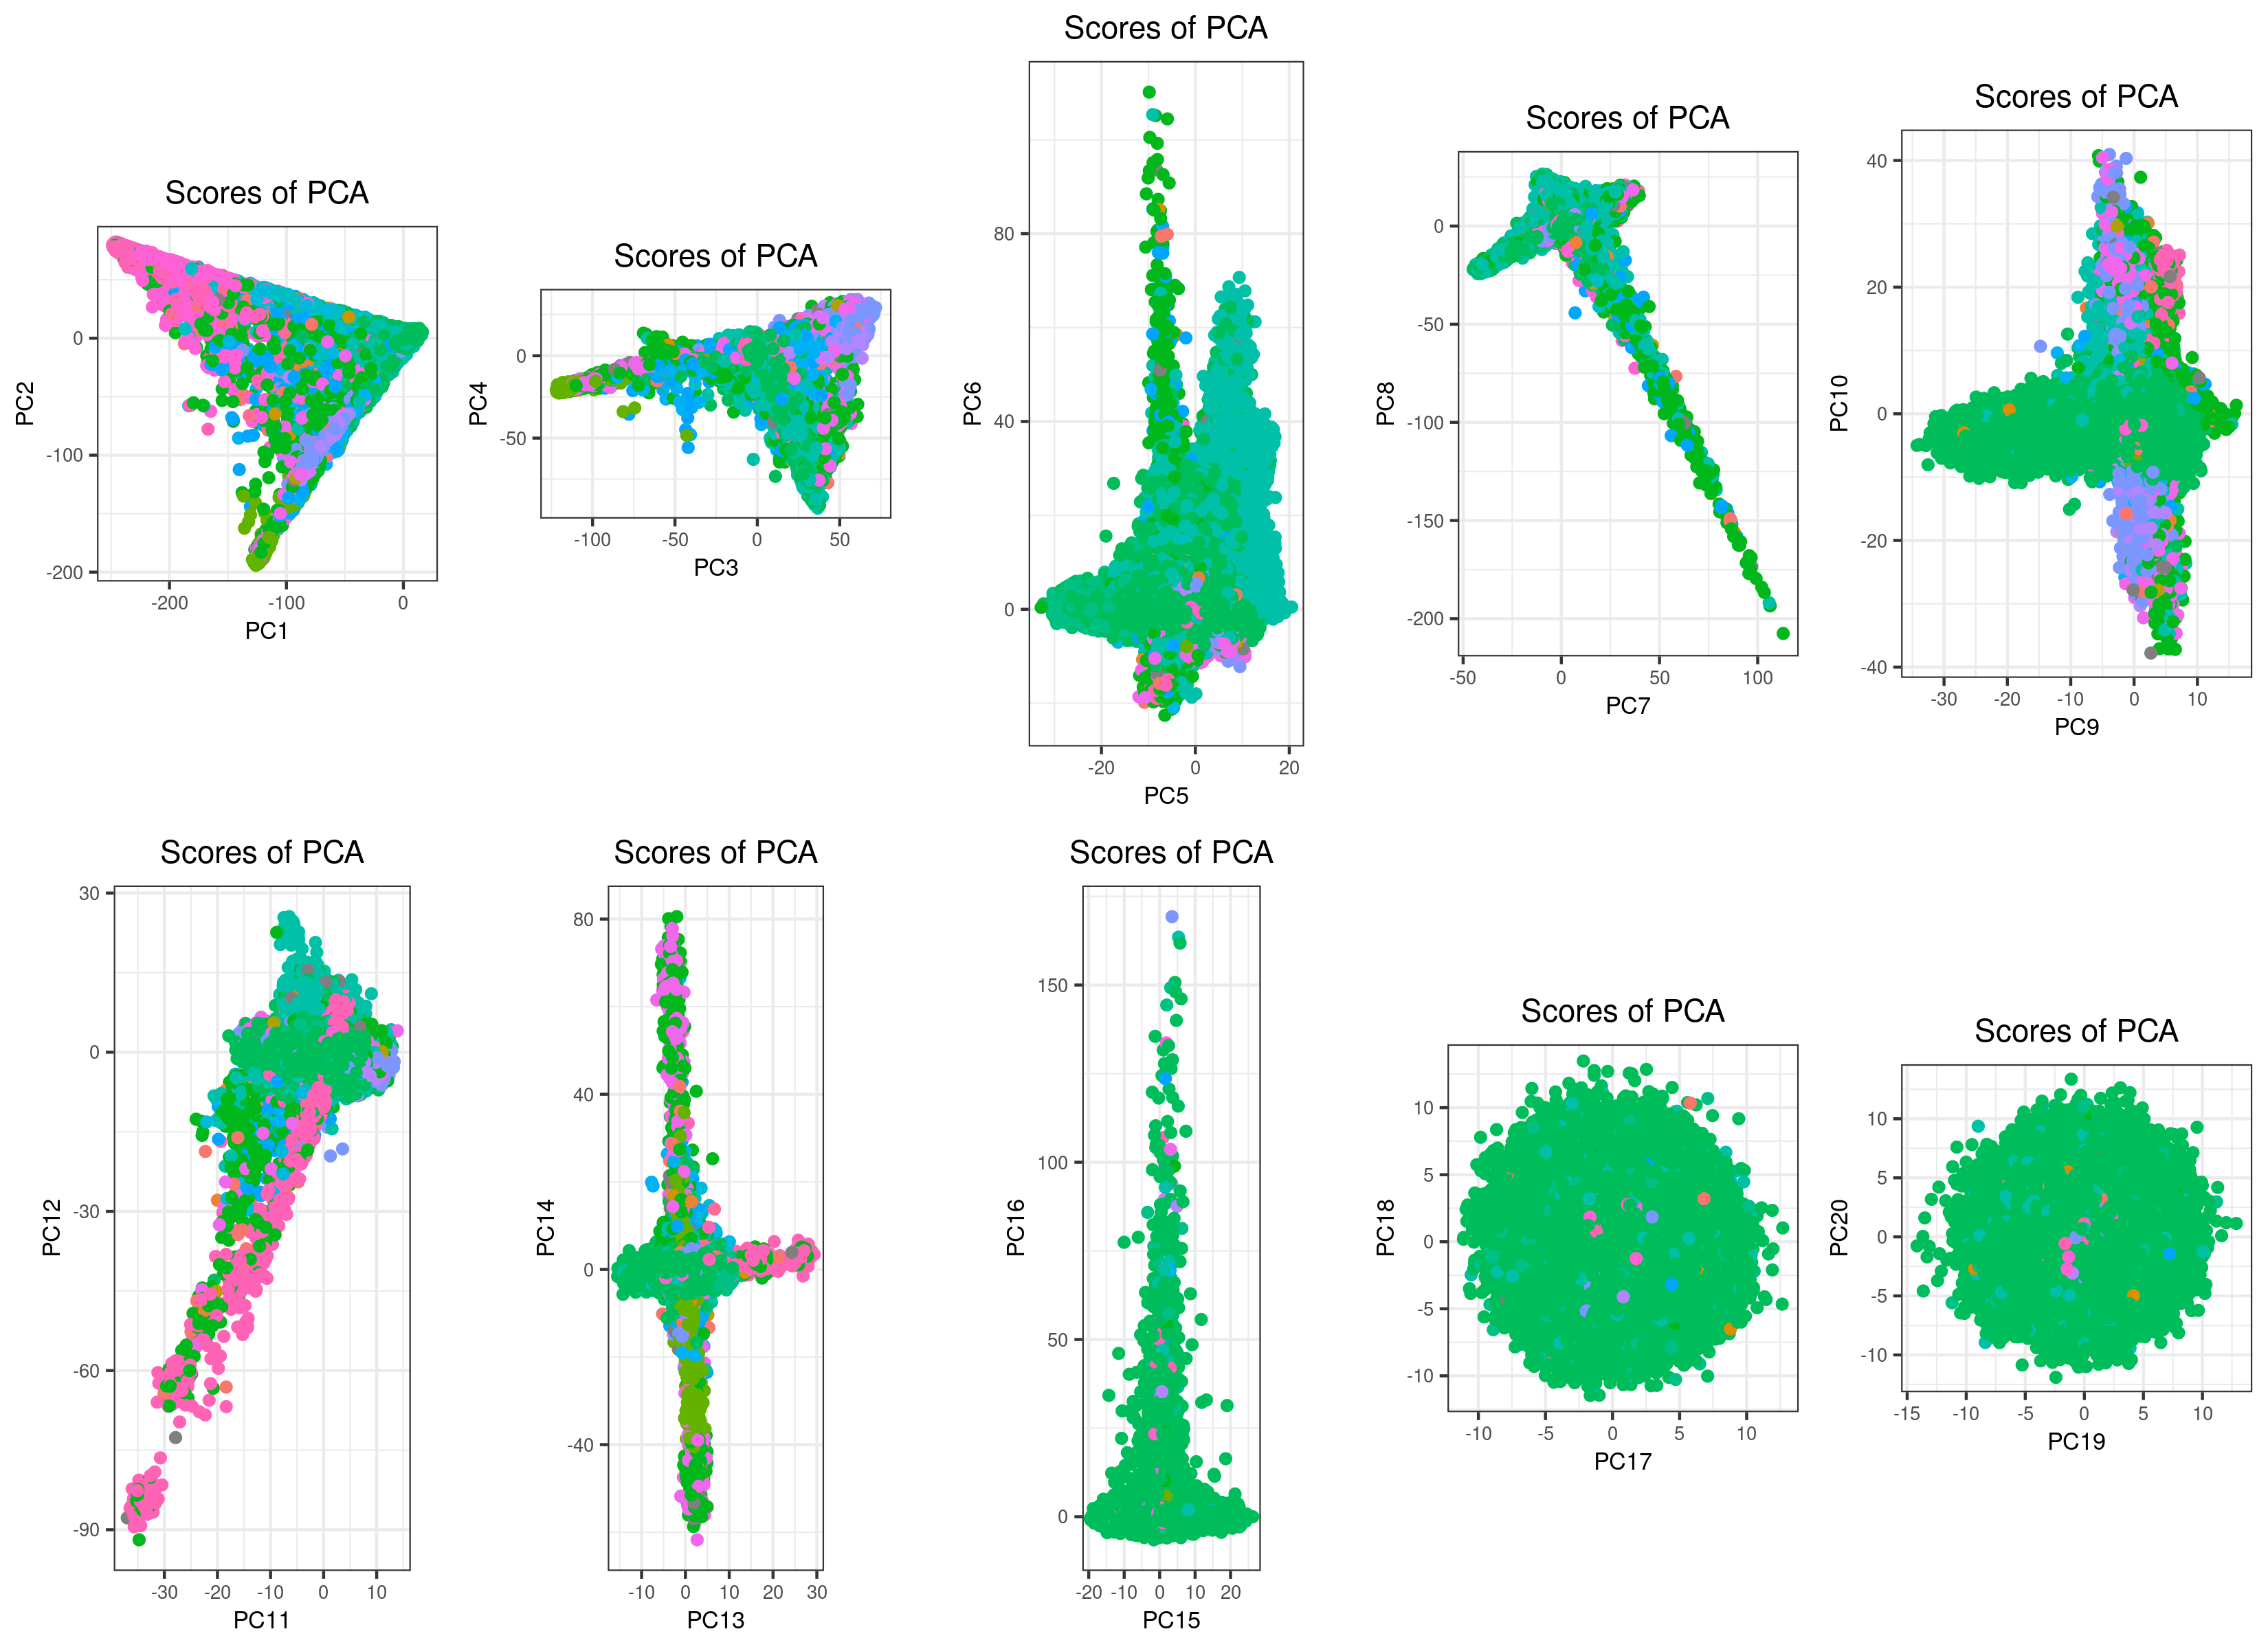
\includegraphics[width=0.9\textwidth]{UKBB-PC1-20.png}}
\caption{Principal Component (PC) scores 1 to 20 computed from the UK Biobank.
\label{fig:UKBB-scores}}
\end{figure}

\begin{figure}[!htpb]
\centerline{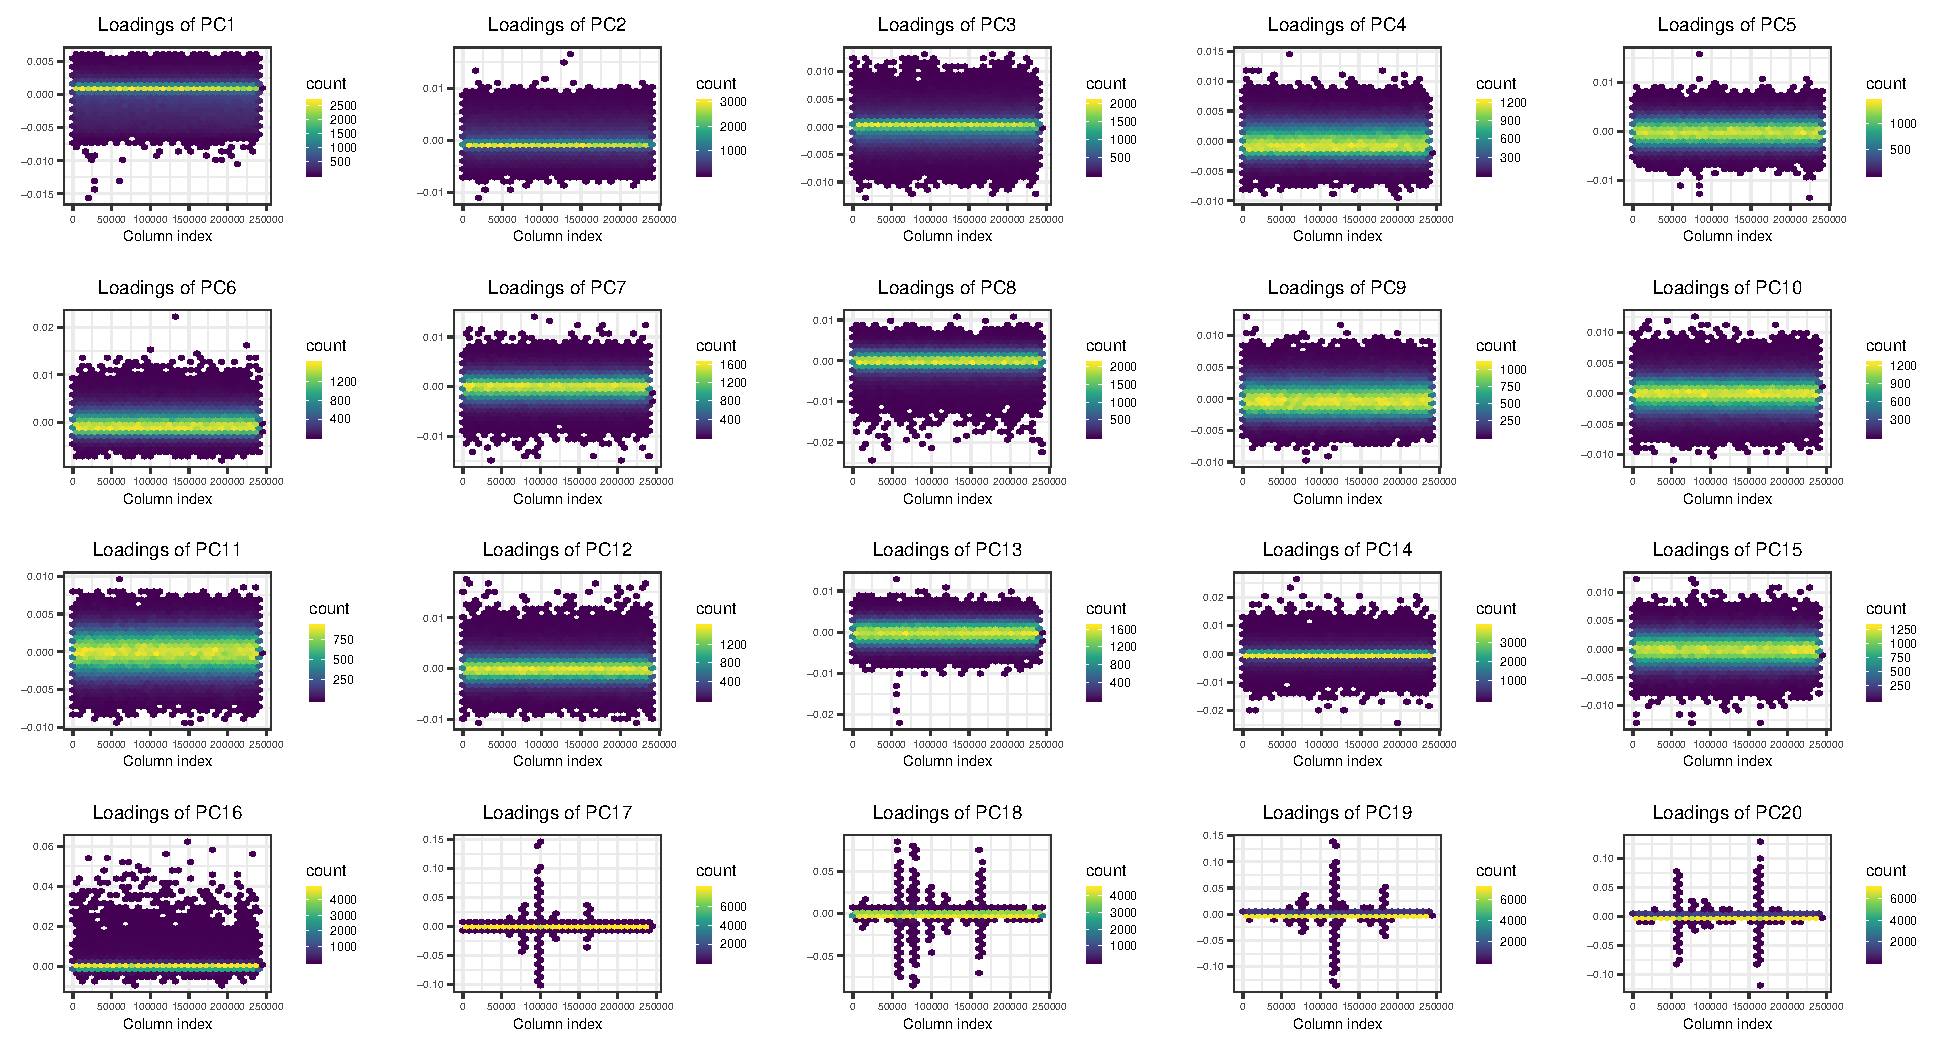
\includegraphics[width=0.9\textwidth]{UKBB-loadings.pdf}}
\caption{Principal Component (PC) loadings 1 to 20 computed from the UK Biobank.
\label{fig:UKBB-loadings}}
\end{figure}

%%%%%%%%%%%%%%%%%%%%%%%%%%%%%%%%%%%%%%%%%%%%%%%%%%%%%%%%%%%%%%%%%%%%%%%%%%%%%%%%

\begin{figure}[!htpb]
\centerline{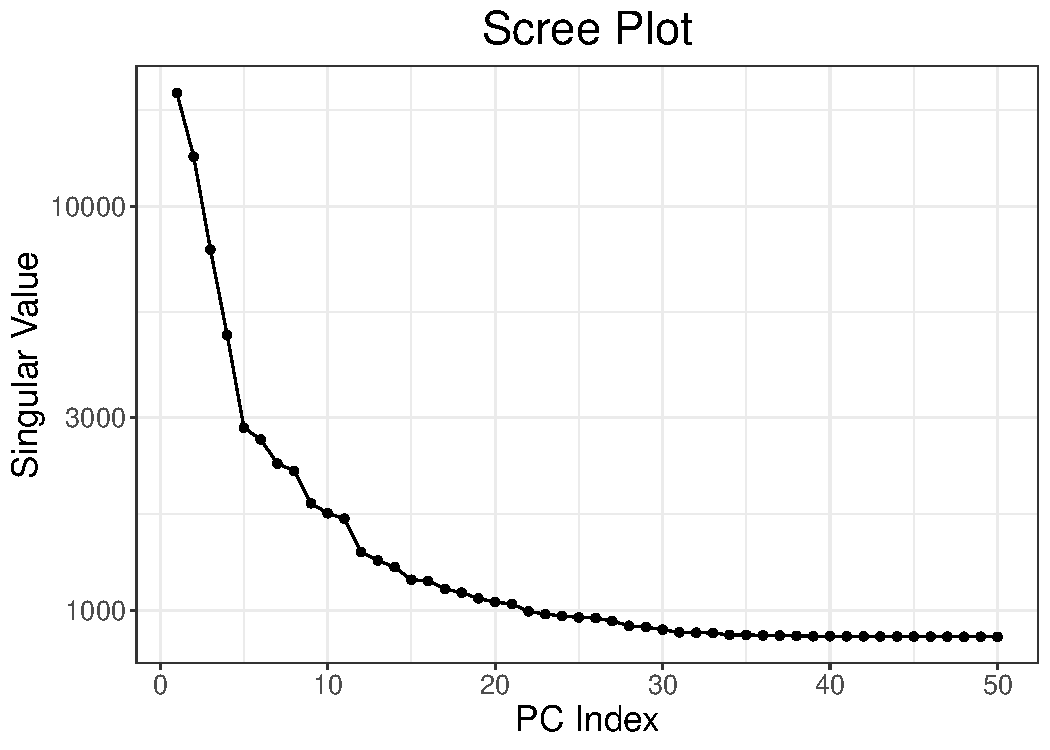
\includegraphics[width=0.8\textwidth]{UKBB-screeplot-restricted.pdf}}
\caption{Scree plot: plot of singular values computed from the UK Biobank using 48,942 individuals of diverse ancestries.
\label{fig:UKBB-screeplot2}}
\end{figure}

\begin{figure}[!htpb]
\centerline{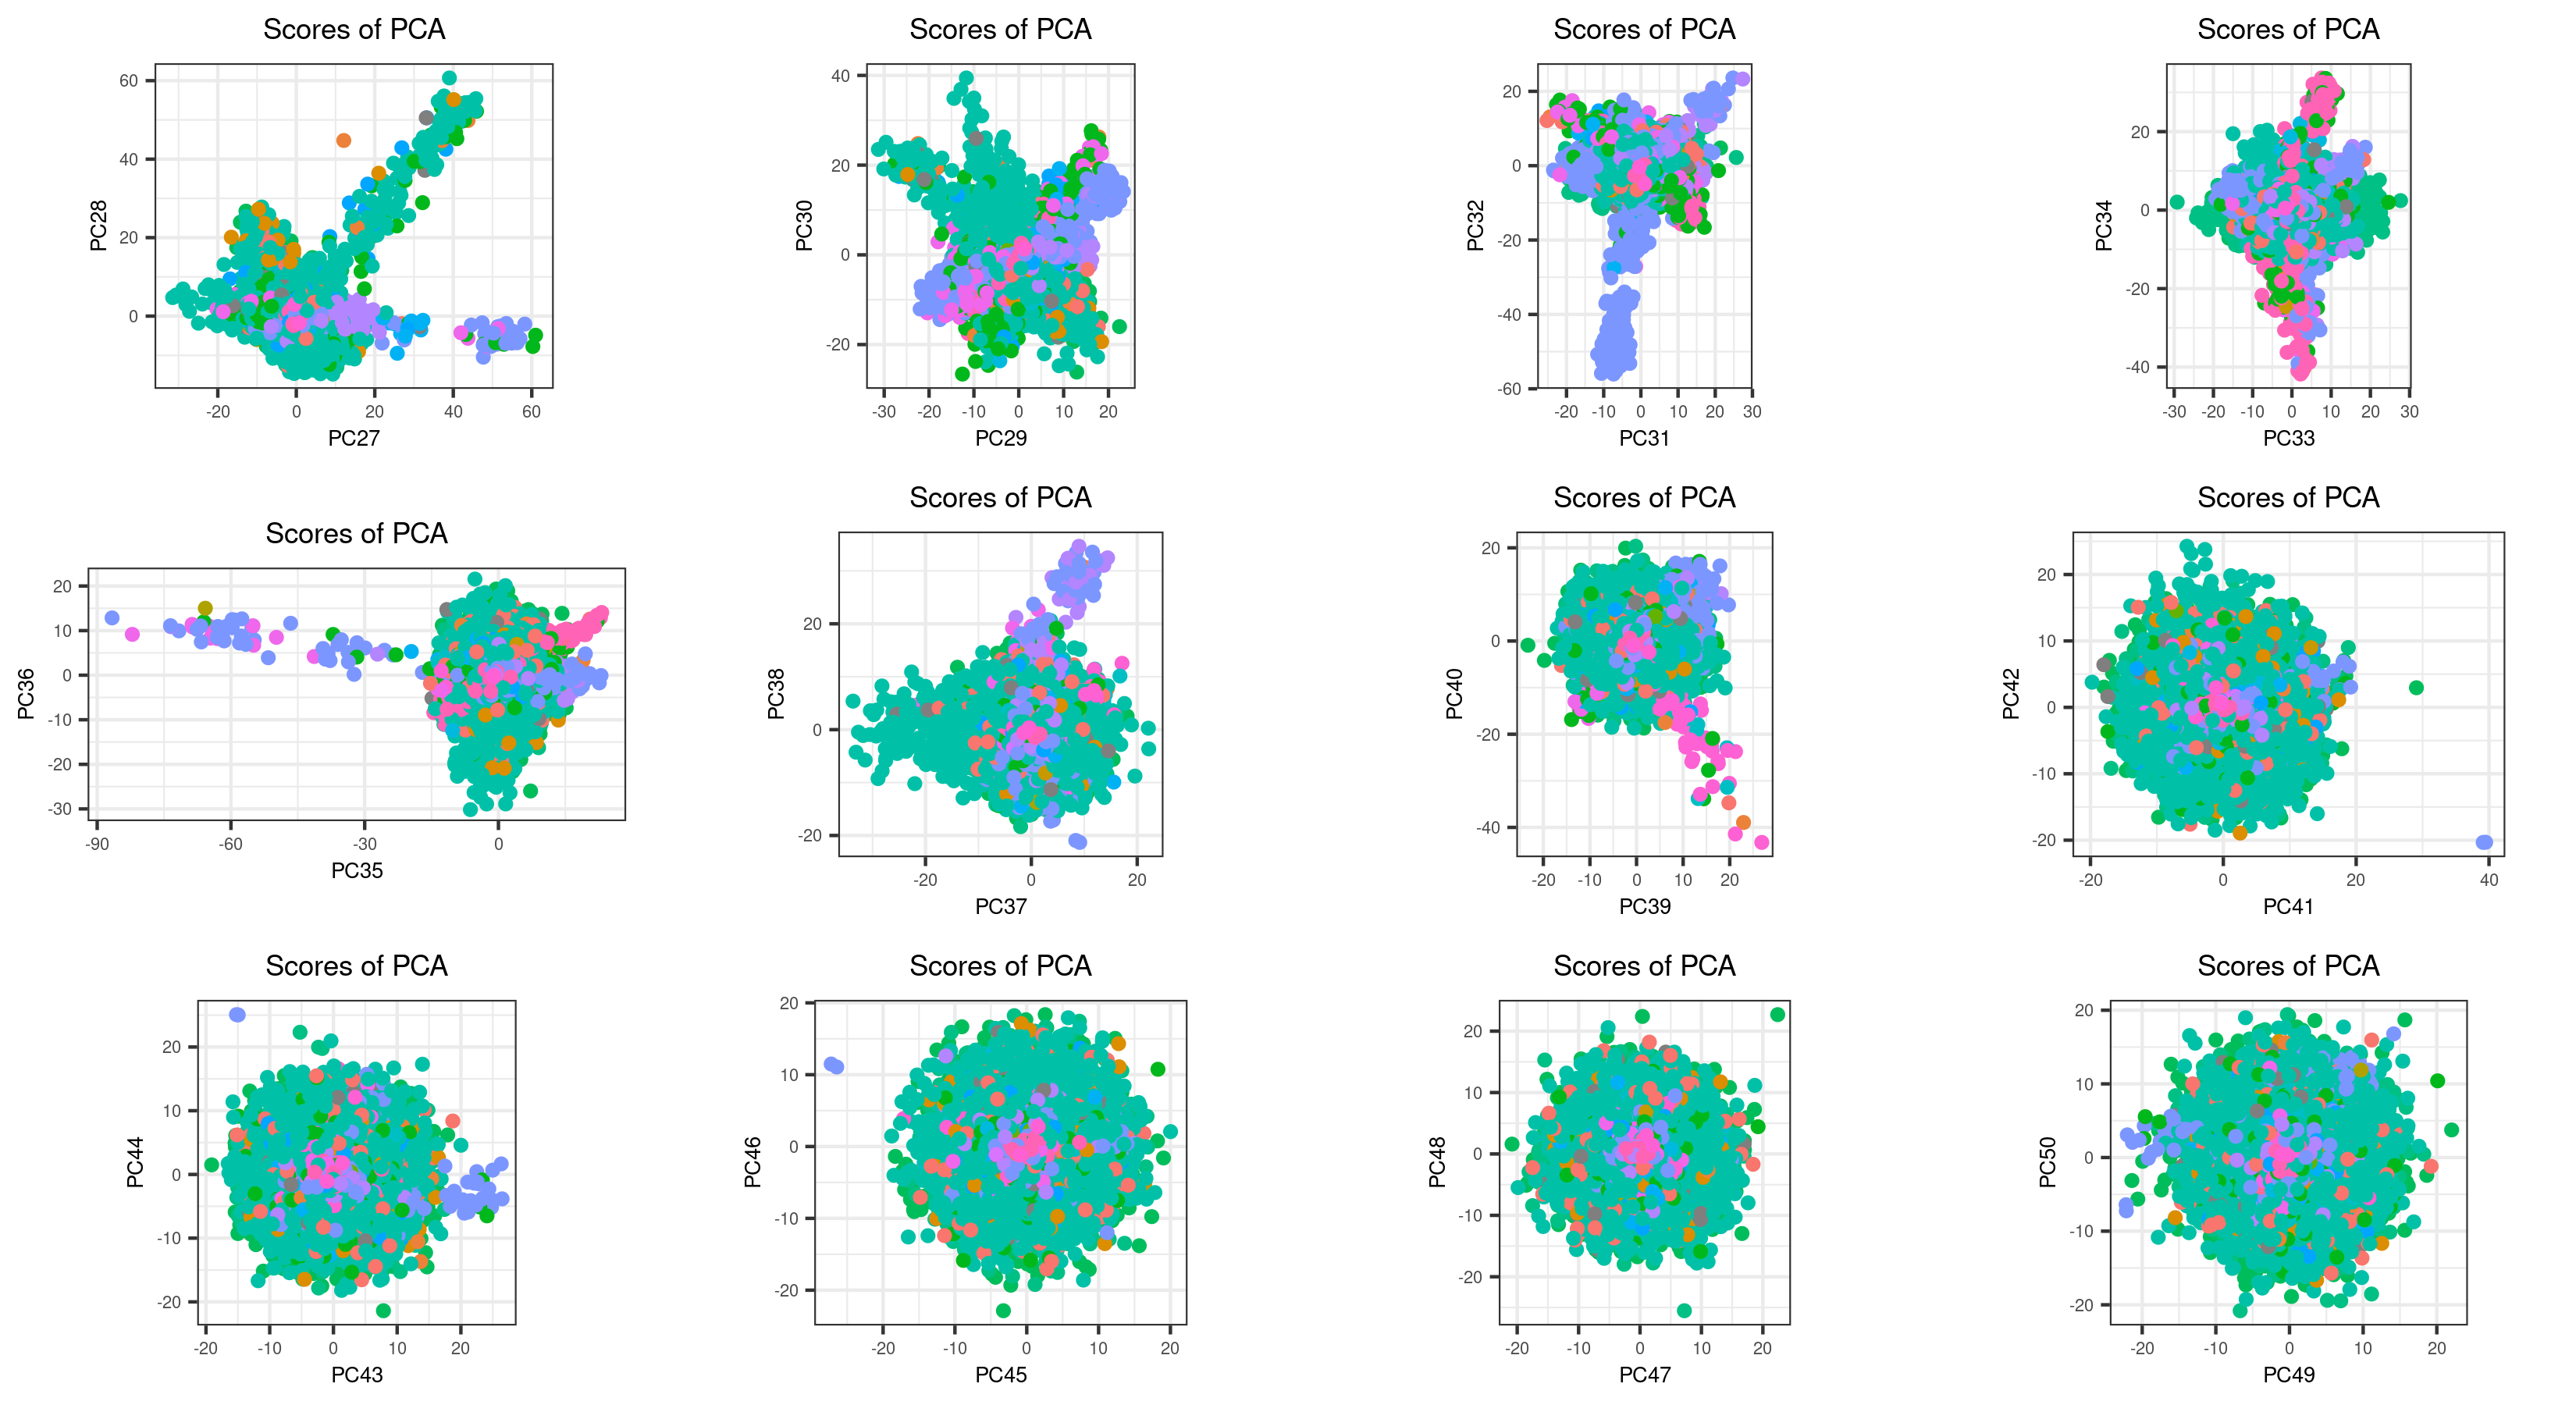
\includegraphics[width=0.9\textwidth]{UKBB-scores-restricted.png}}
\caption{Principal Component (PC) scores 27 to 50 computed from the UK Biobank using 48,942 individuals of diverse ancestries. Different colors represent different self-reported ancestries.
\label{fig:UKBB-scores2}}
\end{figure}

\begin{figure}[!htpb]
\centerline{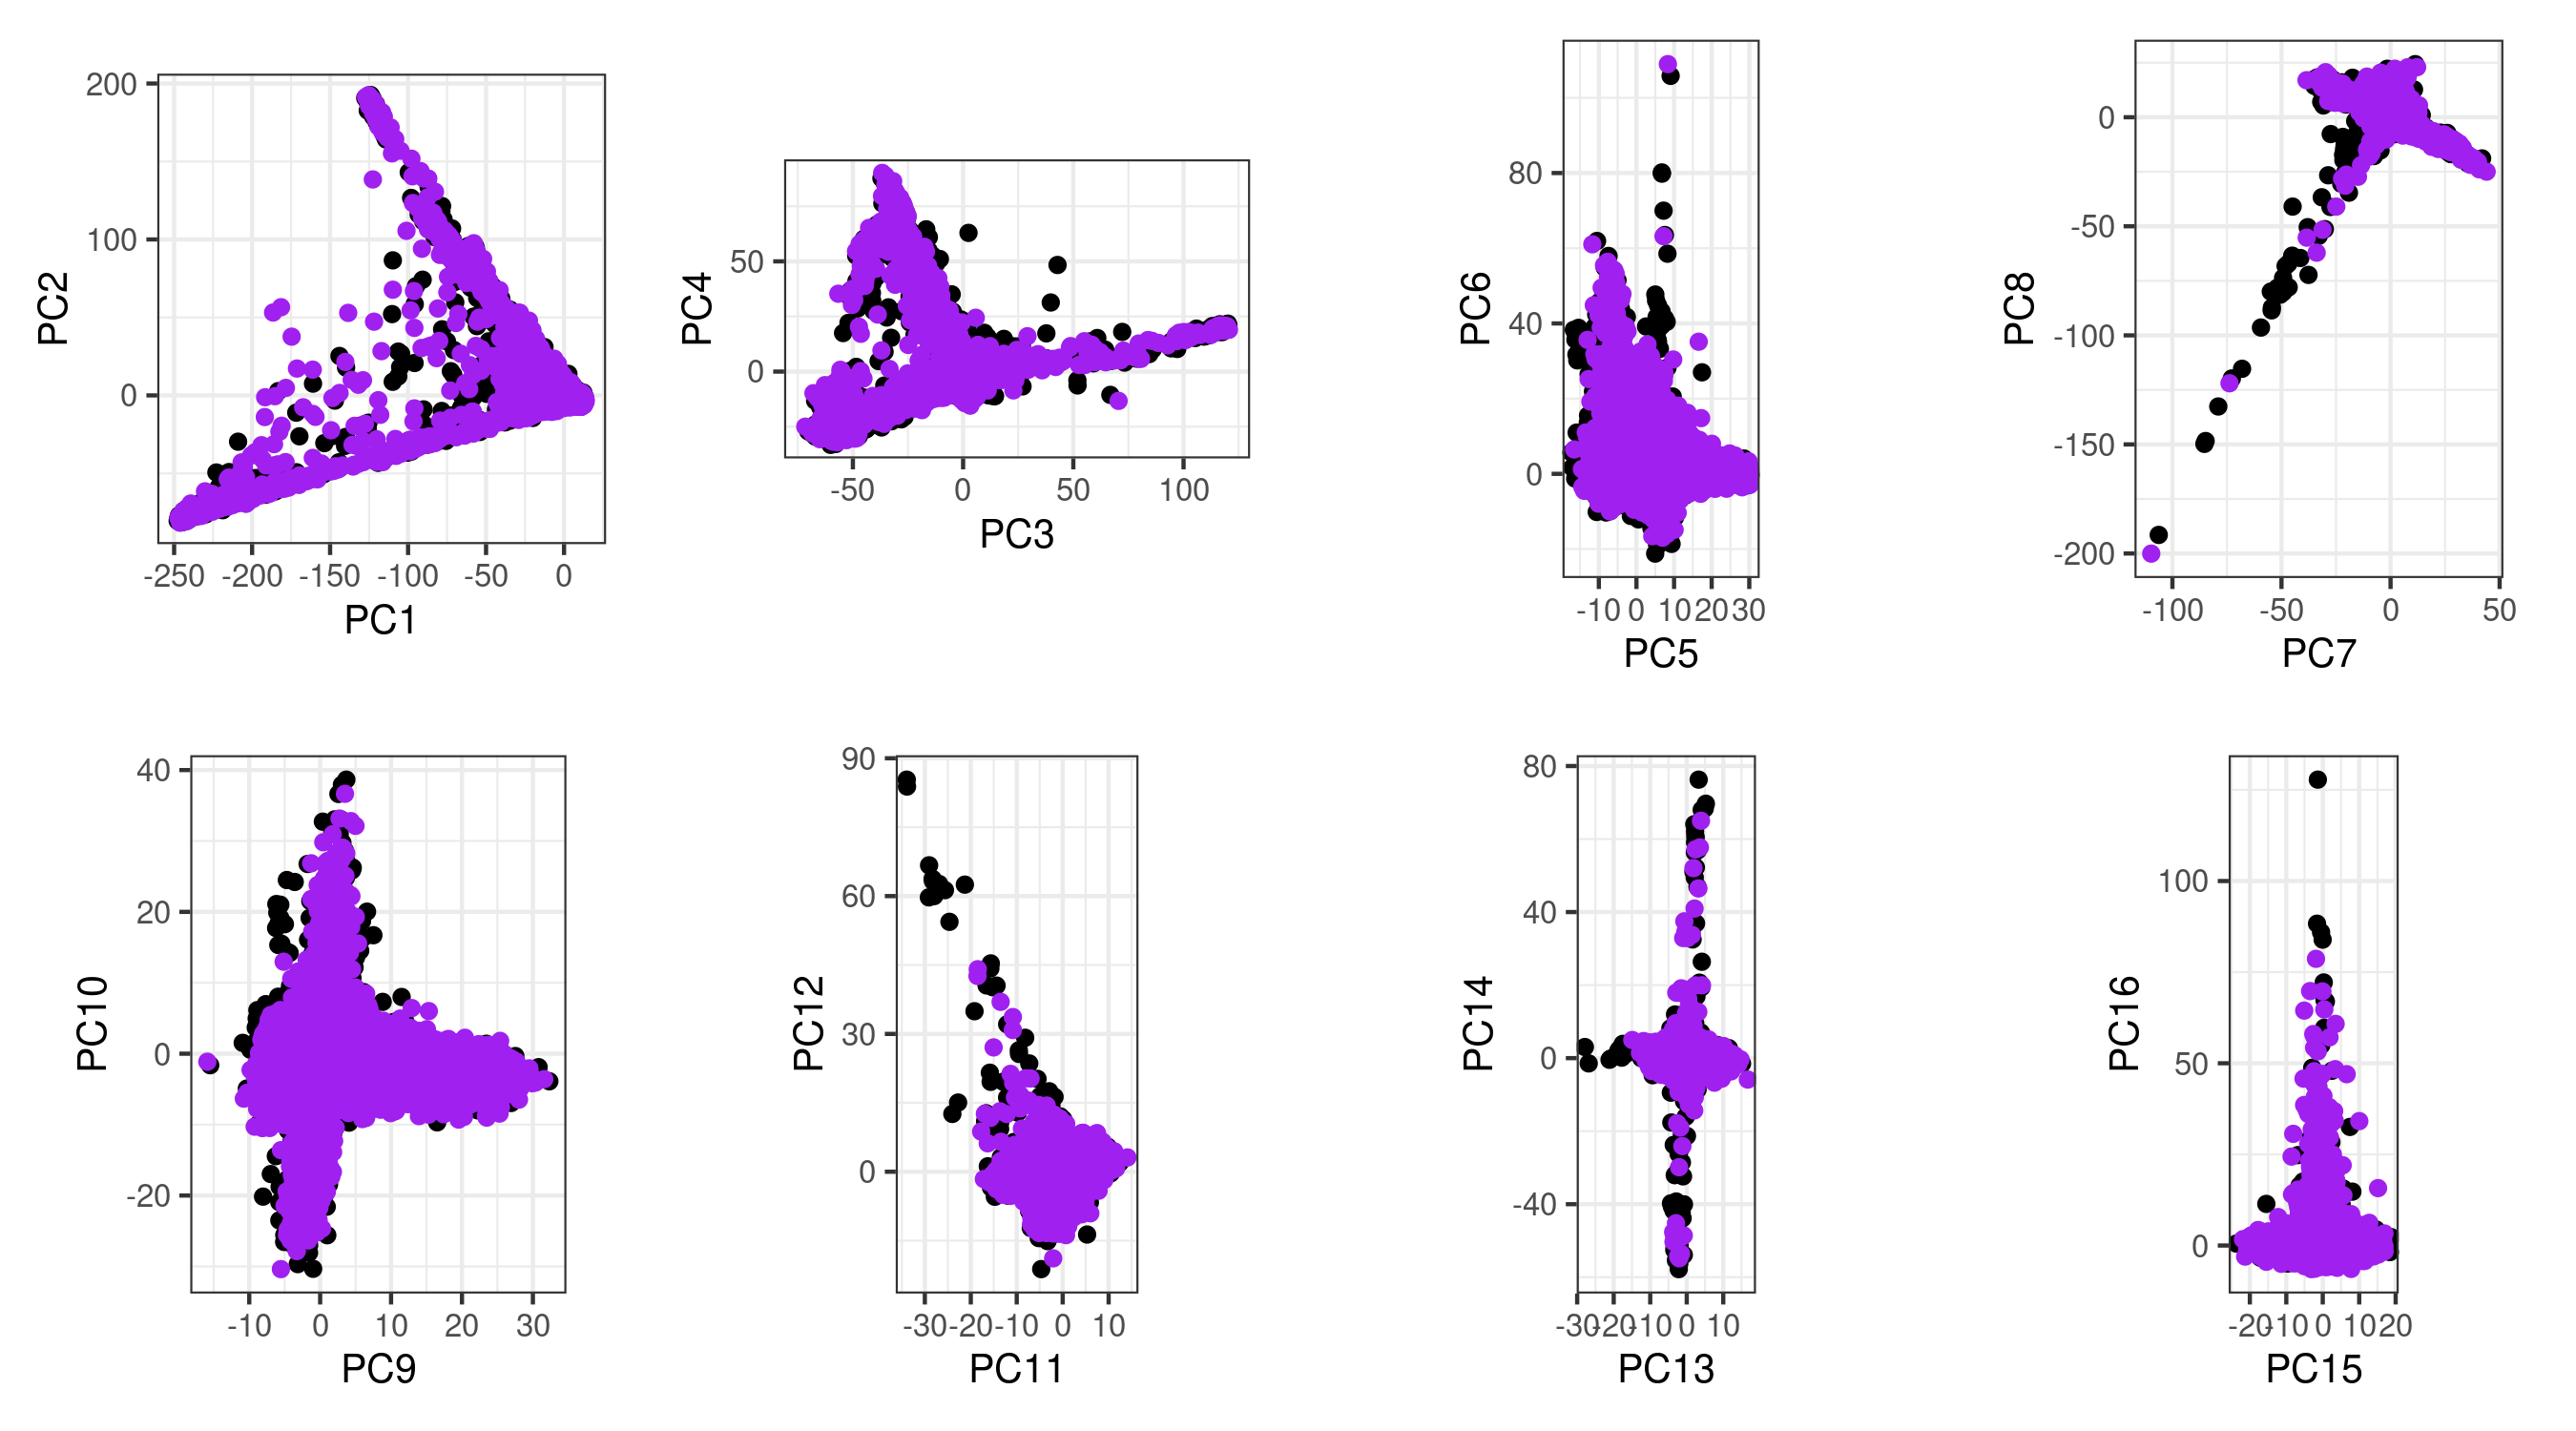
\includegraphics[width=0.9\textwidth]{projUKBB-related.png}}
\caption{Principal Component (PC) scores 27 to 50 of the UK Biobank.
Black points are the 48,942 individuals of diverse ancestries used for computing PCA.
Red points are the remaining UKBB individuals, projected by simply multiplying their genotypes by the corresponding PC loadings.
Blue points are the remaining UKBB individuals, projected using the Online Augmentation, Decomposition, and Procrustes (OADP) transformation.
Note that only 20,000 random projected individuals are represented in this plot.
\label{fig:projUKBB-related}}
\end{figure}

%%%%%%%%%%%%%%%%%%%%%%%%%%%%%%%%%%%%%%%%%%%%%%%%%%%%%%%%%%%%%%%%%%%%%%%%%%%%%%%%

\end{document}
